\documentclass[../main.tex]{subfiles}

\begin{document}

\chapter{入门}
\vspace{-2cm}

本部分为 BasicSR 方法的入门部分,主要涉及的有目录解读,核心的工程文件以及其内部运行的逻辑关系,训练,测试和快速推理的流程。这个部分的主要介绍目的是希望读者能够快速的掌握BasicSR的整体结构用于自己开发使用。

% ------------------------------------------------------------------------------

\section{目录解读}\label{getting_start:content-overview}

所谓“看书先看目录”。我们首先来看一下 BasicSR 仓库的基本结构,先来整体地把握一下。根据仓库的目录层级,第一部分为仓库的整体概览。这部分主要包括算法核心文件和代码基础配置文件。具体的目录结构如下。

其中,\newline
\noindent\textcolor{red}{红色} 表示和跑实验直接相关的文件,即我们平时打交道最多的文件;\newline
\noindent\textcolor{blue}{蓝色} 表示其他与 BasicSR 强相关的代码文件;\newline
\noindent\textcolor{black}{黑色} 表示配置文件。

\vspace{0.5cm}
\renewcommand*\DTstyle{\ttfamily\textcolor{black}}
\dirtree{%
    .1 \textcolor{orange}{BasicSR 根目录}.
    .2 .github/workflows\DTcomment{GitHub 的自动 workflows,比如 PyLint、PyPI Publish等}.
    .2 .vscode\DTcomment{VSCode 配置,用于统一格式}.
    .2 LICENSE\DTcomment{使用的其他代码的 LICENSE 和 Acknowledgement}.
    .2 assets\DTcomment{存放仓库中展示使用的图片}.
    .2 \uline{\textcolor{red}{basicsr}}\DTcomment{\textcolor{red}{BasicSR 核心代码}}.
    .2 \textcolor{blue}{colab}\DTcomment{\textcolor{blue}{Google Colab 的 Notebook, 提供方便的 inference demo}}.
    .2 \textcolor{red}{datasets}\DTcomment{\textcolor{red}{“存放”使用的数据集,推荐 soft link,做到代码、数据的分离}}.
    .2 docs\DTcomment{使用和说明文档}.
    .2 \textcolor{red}{experiments}\DTcomment{\textcolor{red}{实验 checkpoints 保存路径}}.
    .3 \textcolor{blue}{pretrained\_models}\DTcomment{\textcolor{blue}{预训练模型存放路径}}.
    .2 \textcolor{red}{inference}\DTcomment{\textcolor{red}{快速推理,主要用于得到 demo 结果}}.
    .2 \uline{\textcolor{red}{options}}\DTcomment{\textcolor{red}{训练和测试的配置文件}}.
    .2 \uline{\textcolor{red}{scripts}}\DTcomment{\textcolor{red}{功能脚本,包含数据集制作,指标测试和数据集下载等}}.
    .2 \textcolor{blue}{test\_scripts}\DTcomment{\textcolor{blue}{一些用于手动单元测试的脚本}}.
    .2 \textcolor{blue}{tests}\DTcomment{\textcolor{blue}{PyTest 自动单元测试}}.
    .2 .gitignore\DTcomment{Git 忽略文件的配置}.
    .2 .pre-commit-config.yaml\DTcomment{Pre-commit Hook 的配置文件}.
    .2 .readthedocs.yaml\DTcomment{自动触发 basicsr.readthedocs.io 的配置文件}.
    .2 MANIFEST.in\DTcomment{发布 basicsr 时,额外需要包含进去的文件}.
    .2 README.md\DTcomment{说明文档}.
    .2 README\_CN.md\DTcomment{说明文档中文版}.
    .2 \textcolor{blue}{VERSION}\DTcomment{\textcolor{blue}{版本文件}}.
    .2 \textcolor{blue}{requirements.txt}\DTcomment{ \textcolor{blue}{安装依赖包文件}}.
    .2 setup.cfg\DTcomment{格式配置文件,比如 flake8,yapf 和 isort}.
    .2 \textcolor{blue}{setup.py}\DTcomment{\textcolor{blue}{安装文件}}.
}

\vspace{0.5cm}

在 BasicSR 仓库中,核心代码在 basicsr 这个文件夹中。这个部分主要为深度学习模型常用的代码文件,比如网络结构,损失函数和数据加载等,具体目录如下。

其中,\textcolor{red}{红色} 表示我们在开发中主要修改的文件。

\vspace{0.5cm}
\dirtree{%
    .1 \textcolor{orange}{basicsr}.
    .2 \textcolor{red}{archs}\DTcomment{\textcolor{red}{定义网络结构和 forward 的步骤}}.
    .2 \textcolor{red}{data}\DTcomment{\textcolor{red}{定义 Dataset 来喂给模型的训练,Dataloader 的定义也在这里}}.
    .2 losses\DTcomment{定义损失函数}.
    .2 metrics\DTcomment{定义评价指标,比如 PSNR,SSIM,NIQE 等}.
    .2 \textcolor{red}{models}\DTcomment{\textcolor{red}{定义一次完整训练,比如前向、反向传播,梯度优化,Validation等}}.
    .2 ops\DTcomment{定义需要编译的算子,例如 StyleGAN 中用到的算子等}.
    .2 utils\DTcomment{定义基础工具,例如 file client,logger,registry,image process,matlab function等}.
    .2 \textcolor{blue}{test.py}\DTcomment{\textcolor{blue}{定义测试流程,是测试文件的主文件、入口}}.
    .2 \textcolor{blue}{train.py}\DTcomment{\textcolor{blue}{定义训练流程,是训练文件的主文件、入口}}.
}

\vspace{0.5cm}

由于在算法设计和开发中,还需要用到一些脚本,比如数据的预处理、指标计算等,相关的文件位于scripts,目录如下:
\vspace{0.5cm}

\dirtree{%
    .1 \textcolor{orange}{scripts}.
    .2 data\_preparation\DTcomment{准备数据}.
    .2 matlab\_scripts\DTcomment{基于 MATLAB 语言的数据处理脚本}.
    .2 metrics\DTcomment{计算指标的脚本,例如 PSNR,SSIM,NIQE等}.
    .2 model\_conversion\DTcomment{模型转换的脚本,主要是 .pth 文件的 keys 转换}.
    .2 dist\_test.sh\DTcomment{方便的分布式测试启动脚本}.
    .2 dist\_train.sh\DTcomment{方便的分布式训练启动脚本}.
    .2 download\_gdrive.py\DTcomment{从 Google Drive 下载文件的脚本}.
    .2 download\_pretrained\_models.py\DTcomment{从 Google Drive 批量下载预训练模型的脚本}.
    .2 publish\_models\DTcomment{发布模型的脚本,包括添加 SHA 等}.
}

至此,我们对 BasicSR 的整体框架便有了一定的了解啦 $\sim$

% ------------------------------------------------------------------------------

\section{训练流程}\label{getting_start:training_pipeline}

在对目录结构有了初步的了解之后就可以进行训练了。我们希望 BasicSR 即方便使用,又清晰易懂,降低使用者的门槛。但随着 BasicSR 代码库逐渐抽象和复杂起来,很多刚接触的同学不知道程序入口在哪里,数据、模型和网络是在哪里定义的,流程又是在哪里控制的,那么我们就通过一个例子简要地说一下。

本节的目的是希望能够初步地让读者了解到训练的基本流程和代码逻辑流,具体的细节我们会采用引用的方式来供读者查阅。如果你已经熟悉 BasicSR 的主要框架和流程,可以跳过这一章节。

% ----------------------------------
\subsection{代码的入口和训练的准备工作}
我们以训练超分辨率模型 MSRResNet 为例,首先需要在终端输入命令来开始训练:

\begin{minted}[xleftmargin=20pt,breaklines,bgcolor=bg]{bash}
python basicsr/train.py -opt options/train/SRResNet_SRGAN/train_MSRResNet_x4.yml
\end{minted}

它从 basicsr/train.py 的 train\_pipeline 函数作为入口:

\begin{figure}[h]
    \begin{center}
        \vspace{-0.2cm}
        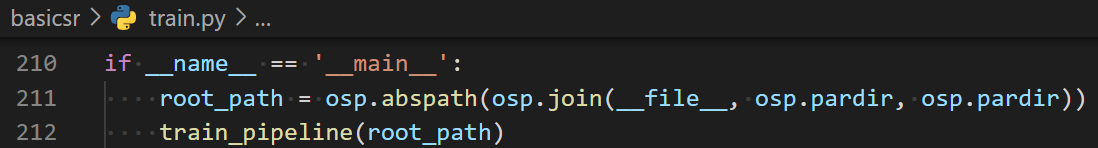
\includegraphics[width=0.9\linewidth]{figures/getting_start_train_entracne.png}
        \vspace{-0.3cm}
        \caption{函数 train\_pipeline 作为 basicsr/train.py 的入口}
        \label{fig:getting_start_train_entracne}
    \end{center}
    \vspace{-0.5cm}
\end{figure}

\begin{exampleBox}[righthand ratio=0.00, sidebyside, sidebyside align=center, lower separated=false]{root\_path 作为参数传进去}
    这里为什么要把root\_path 作为参数传进去呢?是因为,当我们把 basicsr 作为 package 使用的时候,需要根据当前的目录路径来创建文件,否则程序会错误地使用 basicsr package 所在位置的目录了。
\end{exampleBox}

train\_pipeline 函数会做一些基础的事,比如:
\begin{enumerate}
    \item 解析配置文件 option file,即 yml 文件
    \item 设置 distributed training 的相关选项,设置 random seed 等
    \item 如果有 resume,需要 load 相应的状态
    \item 创建相关文件夹,拷贝配置的 yml 文件
    \item 合理初始化日志系统 logger
\end{enumerate}

我们对着代码一一讲解,如图\ref{fig:getting_start_train_pipeline}所示:

\begin{figure}[ht]
    \begin{center}
        \vspace{-0.2cm}
        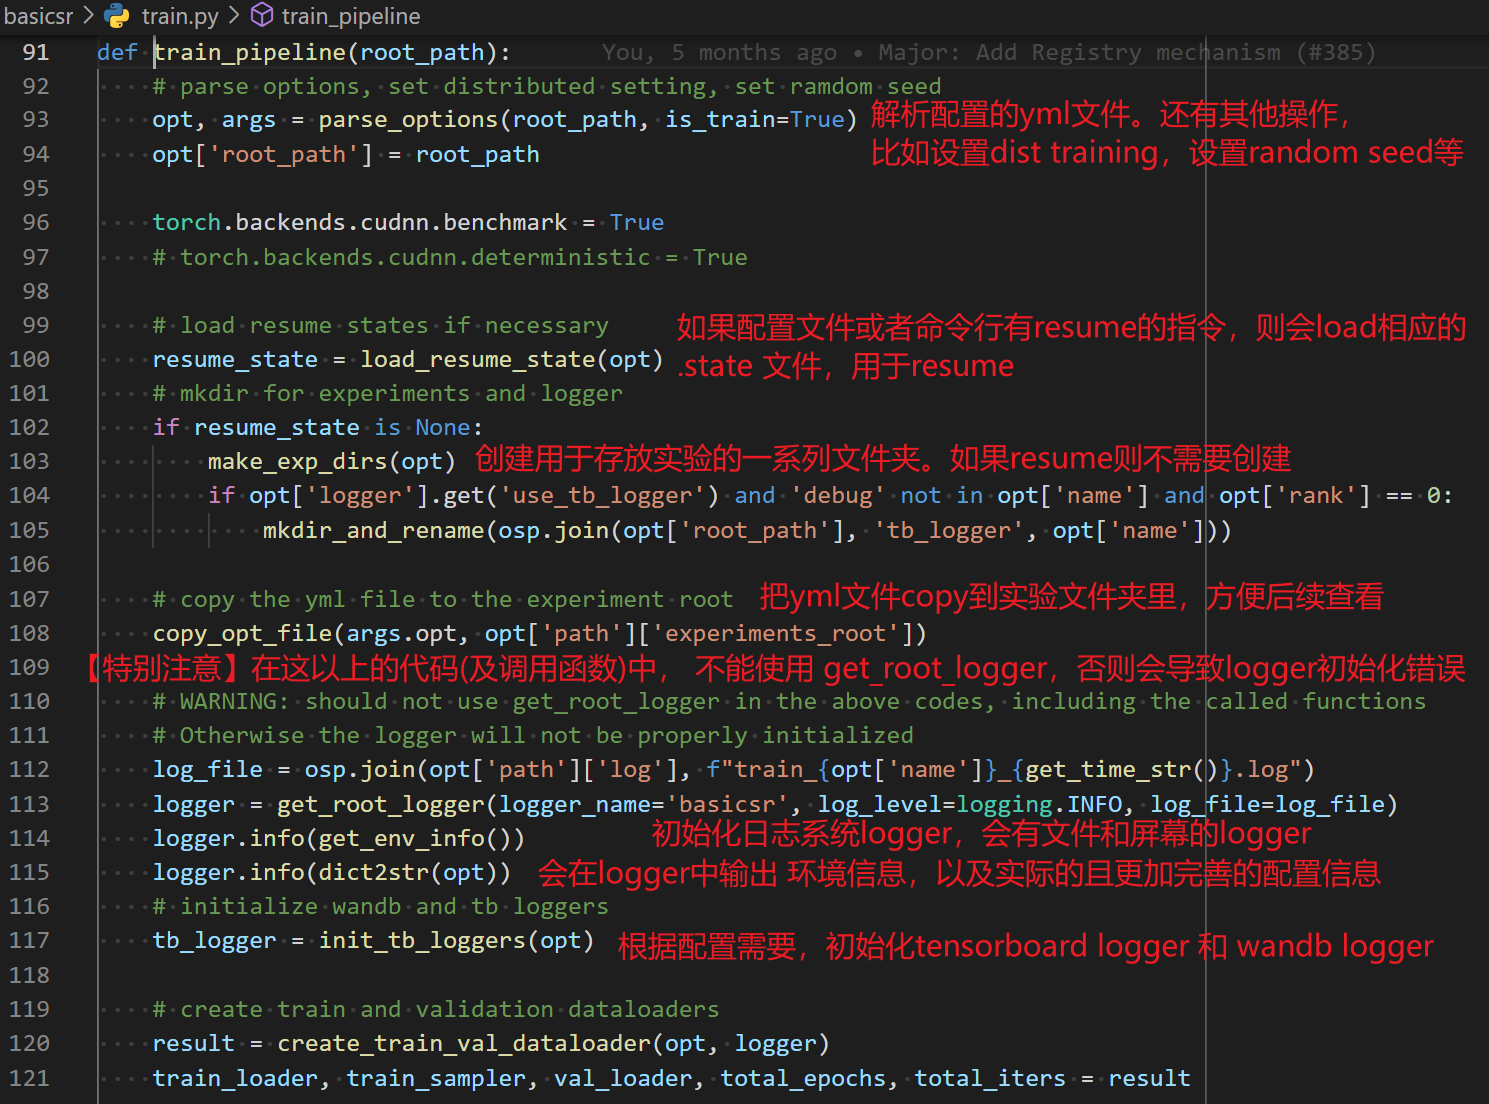
\includegraphics[width=0.9\linewidth]{figures/getting_start_train_pipeline.png}
        \vspace{-0.3cm}
        \caption{函数 train\_pipeline 的基础准备工作}
        \label{fig:getting_start_train_pipeline}
    \end{center}
    \vspace{-0.5cm}
\end{figure}

具体的子函数,大家可以对着代码点进去查看,这里我们着重说几点。

\begin{enumerate}
    \item 我们在命令行中的参数输入,在哪里完成解析呢,即 argparse 在哪里?
          答:是在 parse\_options 这个函数中。我们截取一部分来看一下。

          \begin{figure}[ht]
              \begin{center}
                  \vspace{-0.2cm}
                  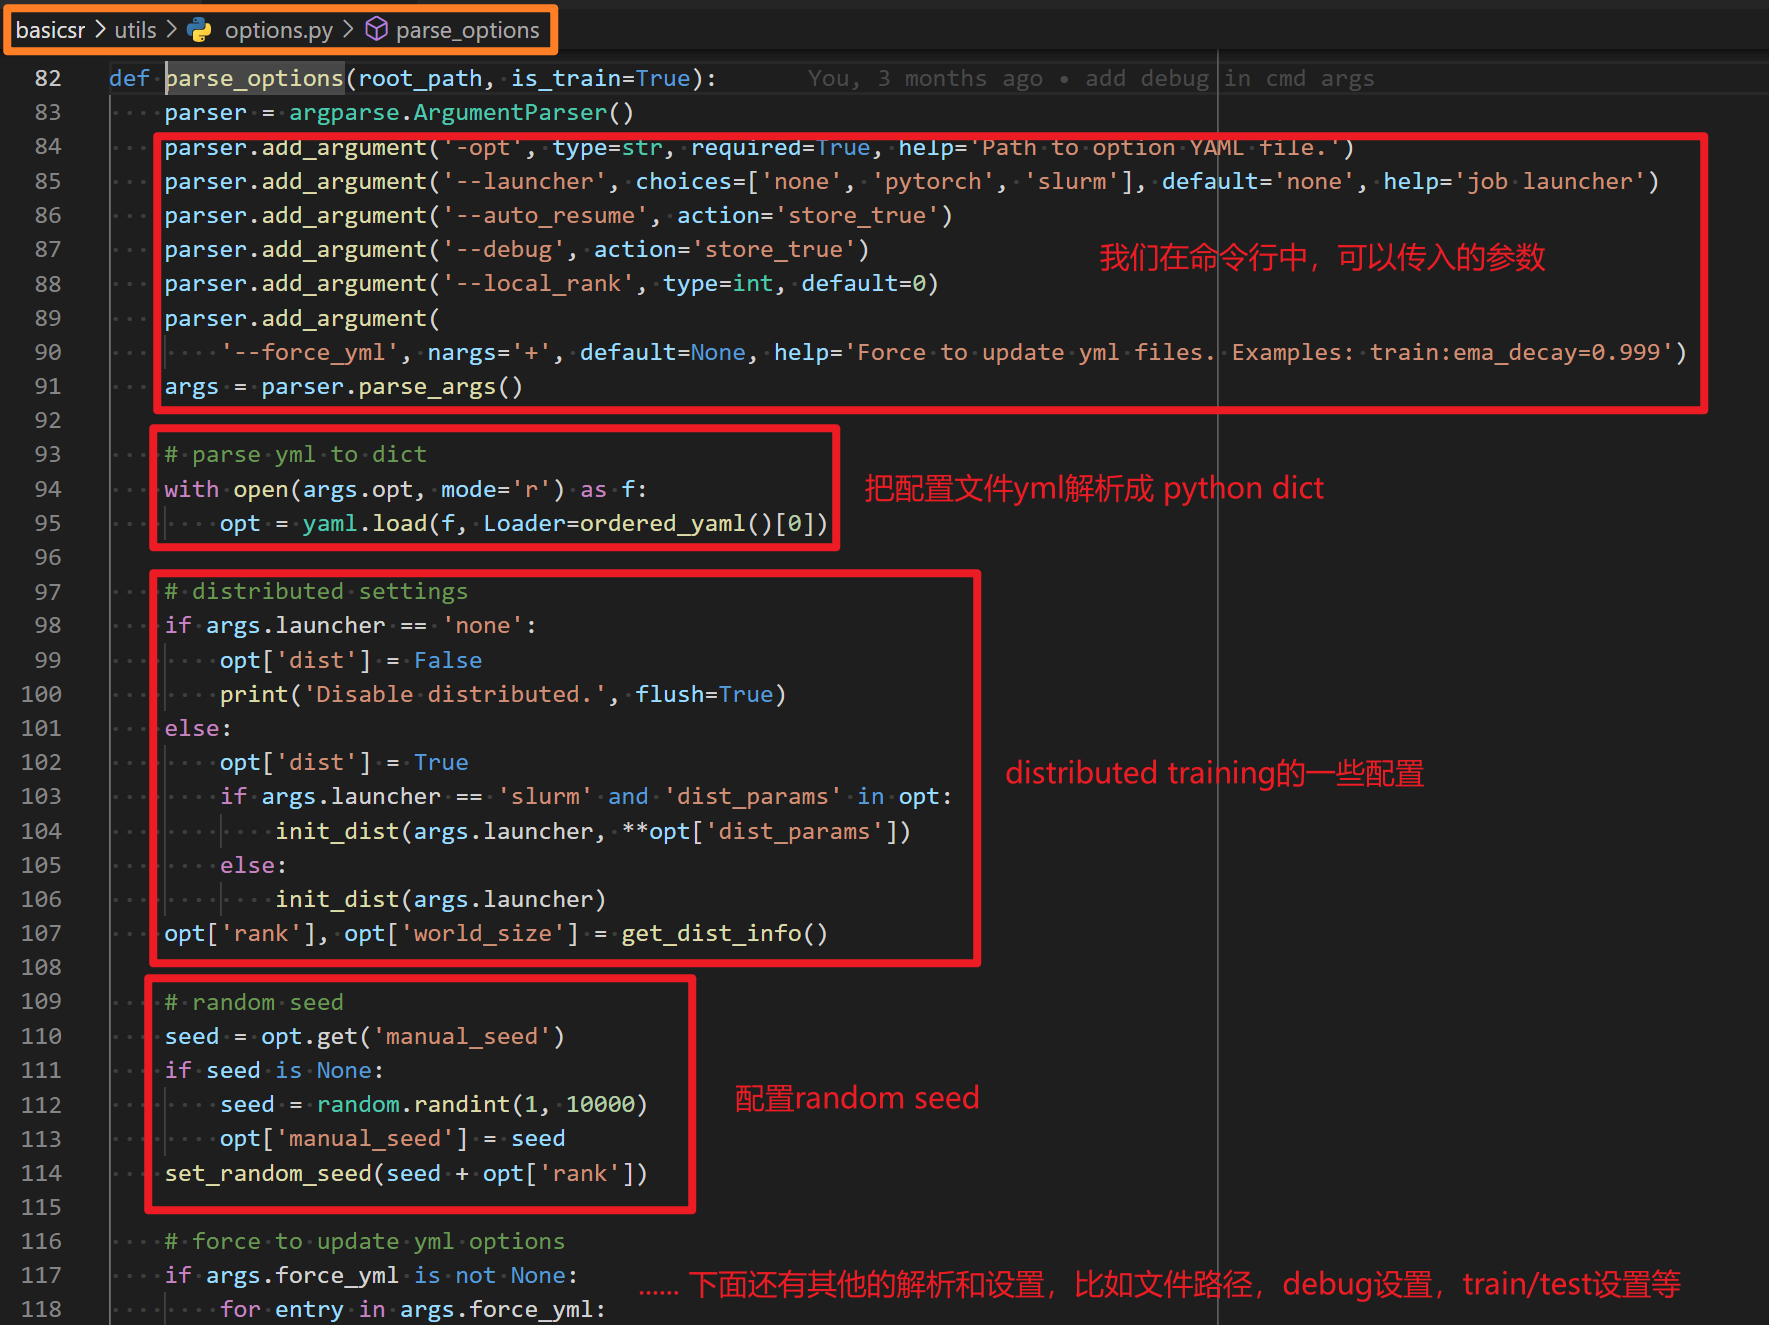
\includegraphics[width=0.9\linewidth]{figures/getting_start_parse_options.png}
                  \vspace{-0.3cm}
                  \caption{函数 parse\_options 解析参数输入}
                  \label{fig:getting_start_parse_options}
              \end{center}
              \vspace{-0.5cm}
          \end{figure}

          从图\ref{fig:getting_start_parse_options}中,我们看到命令行的参数不多。我们一一讲解一下。

          \begin{enumerate}
              \item {-}opt,配置文件的路径,一般采用这个命令配置训练或者测试的 yml 文件。
              \item {-}{-} laucher,用于指定 distibuted training 的,比如 pytorch 或者 slurm。默认是 none,即单卡非 distributed training。
              \item {-}{-} auto\_resume,是否自动 resume,即自动查找最近的 checkpoint ,然后 resume。详见章节\ref{others:auto_resume}:\nameref{others:auto_resume}。
              \item {-}{-} debug,能够快速帮助 debug。详见章节\ref{others:debug_mode}:\nameref{others:debug_mode}。
              \item {-}{-} local\_rank,这个不用管,是 distributed training 中程序自动会传入。
              \item {-}{-} force\_yml,方便在命令行中修改 yml 中的配置文件。详见章节\ref{others:yml_modification_with_commands}:\nameref{others:yml_modification_with_commands}。
          \end{enumerate}


    \item 每个实验创建的文件夹

          每个实验都会在 experiments 目录中创建一个以配置文件中的 name 为名字的文件夹,里面的文件如图\ref{fig:getting_start_exp_folder}所示。log 的内容参见章节\ref{code_structure:logger}:\nameref{code_structure:logger}。在实验文件夹中有把配置文件也 copy 一份,还会额外添加 copy 的时间和运行使用的具体命令,方便事后检查和复现。

          \begin{figure}[h]
              \begin{center}
                  \vspace{-0.2cm}
                  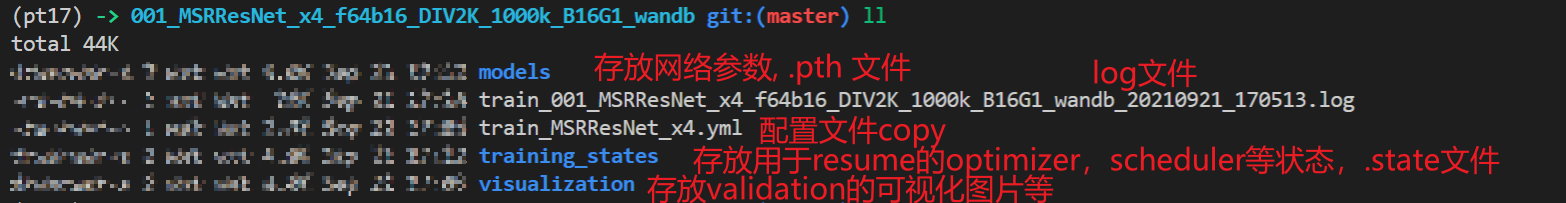
\includegraphics[width=0.9\linewidth]{figures/getting_start_exp_folder.png}
                  \vspace{-0.3cm}
                  \caption{实验过程中创建的文件}
                  \label{fig:getting_start_exp_folder}
              \end{center}
              \vspace{-0.5cm}
          \end{figure}
\end{enumerate}

% ----------------------------------
\subsection{Data 和 Model 的创建}

当训练准备工作结束后,我们接下来就要看 data 和 model 的创建过程了。下图\ref{fig:getting_start_init_data_model}是相对应的代码。
它主要包括:
\begin{enumerate}
    \item 训练和 validation 的 data loader 创建,下面会展开。更多内容参见章节\ref{code_structure:data}:\nameref{code_structure:data}的相关内容
    \item model 的创建
    \item logger 的初始化,这块详见章节\ref{code_structure:logger}:\nameref{code_structure:logger}的相关内容
    \item 还有 dataset prefetch 的内容,这块详见章节\ref{code_structure:data}:\nameref{code_structure:data}的相关内容
\end{enumerate}

\begin{figure}[h]
    \begin{center}
        \vspace{-0.2cm}
        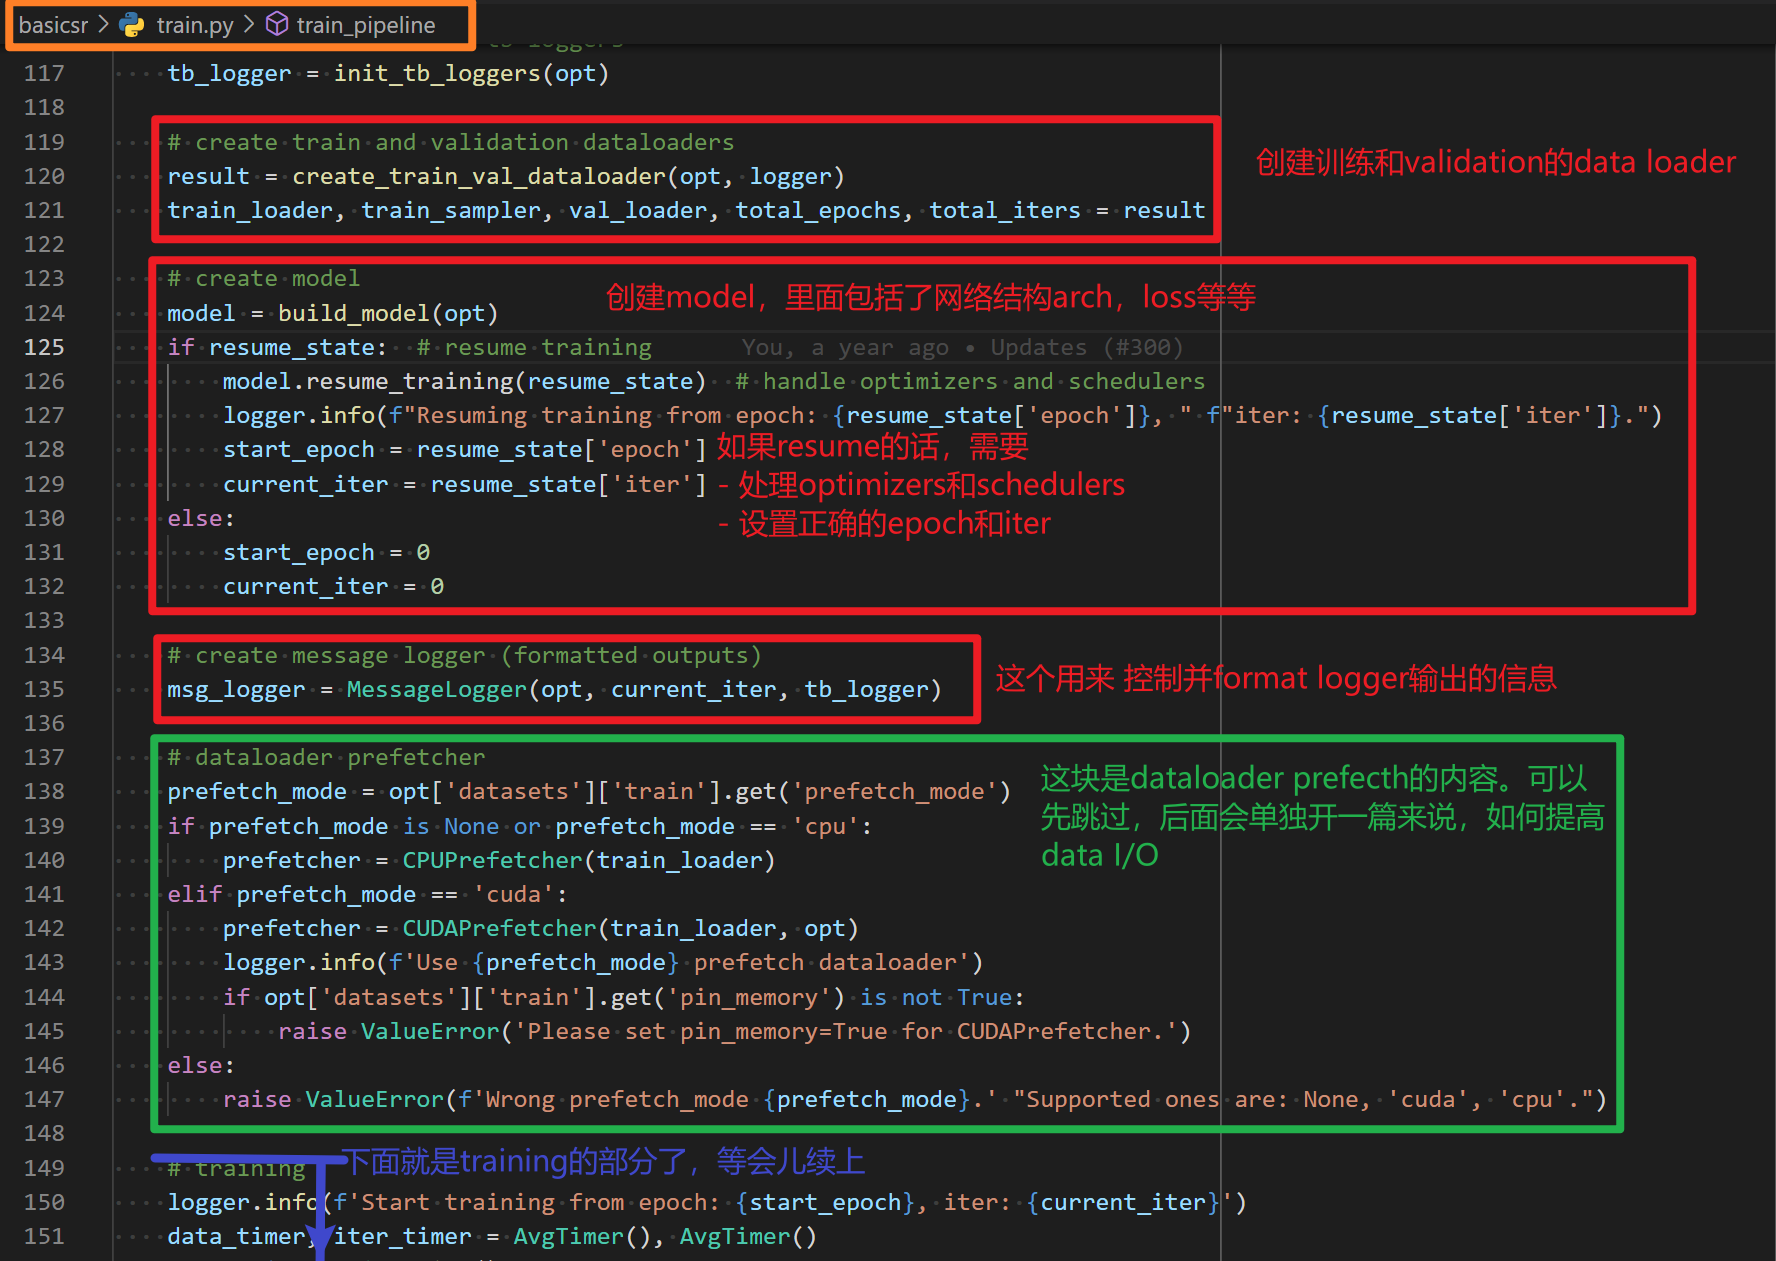
\includegraphics[width=0.9\linewidth]{figures/getting_start_init_data_model.png}
        \vspace{-0.3cm}
        \caption{train\_pipeline 中初始化 data 和 model}
        \label{fig:getting_start_init_data_model}
    \end{center}
    \vspace{-0.5cm}
\end{figure}

这里我们着重讲解两块, dataloader 的创建和 model 的创建。

\begin{enumerate}

    \item dataloader 创建
          首先我们看调用的 create\_train\_val\_dataloader 函数:

          \begin{figure}[H]
              \begin{center}
                  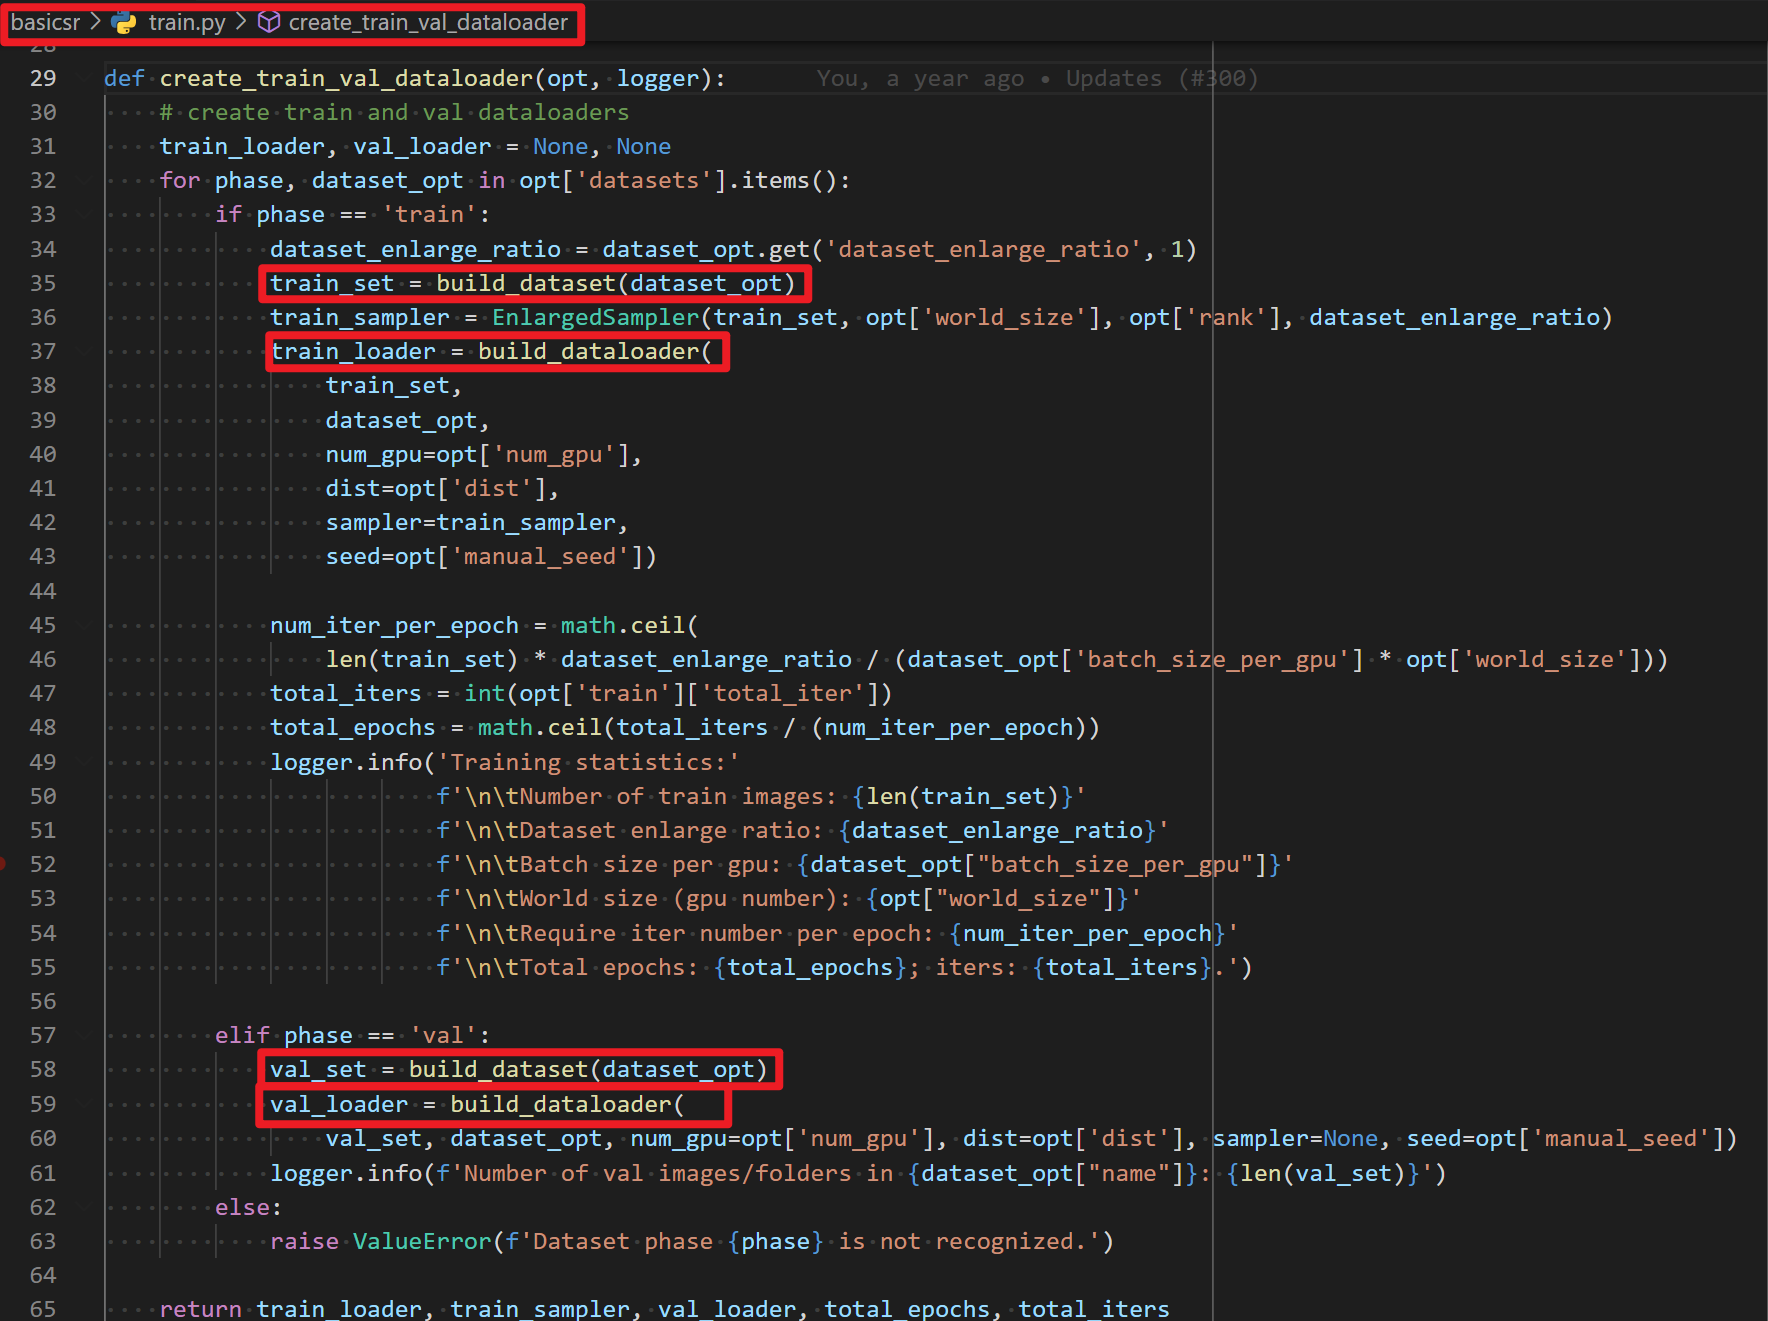
\includegraphics[width=0.7\linewidth]{figures/getting_start_9.png}
                  \caption{初始化 train 和 valid 的 dataloader}
                  \label{fig:getting_start_9}
              \end{center}
              \vspace{-0.5cm}
          \end{figure}

          其他都是细枝末节的,后面可以慢慢看。里面主要的就是两个函数, build\_dataset 和 build\_dataloader 。无论是 train 还是 val 的 dataloader 都是这两个函数构建的。
          创建 dataloder 要靠 build\_dataloader ,其中又要用到 dataset 。而 dataset 是由 build\_dataset 创建的。 dataloder 其实大家都是共用的。当我们说要新写一个 dataloader ,其实写的是 dataset 。 build\_dataloader 和 build\_dataset 都是定义在 basicsr/data/\_\_init\_\_.py 文件里面。

          \begin{figure}[H]
              \begin{center}
                  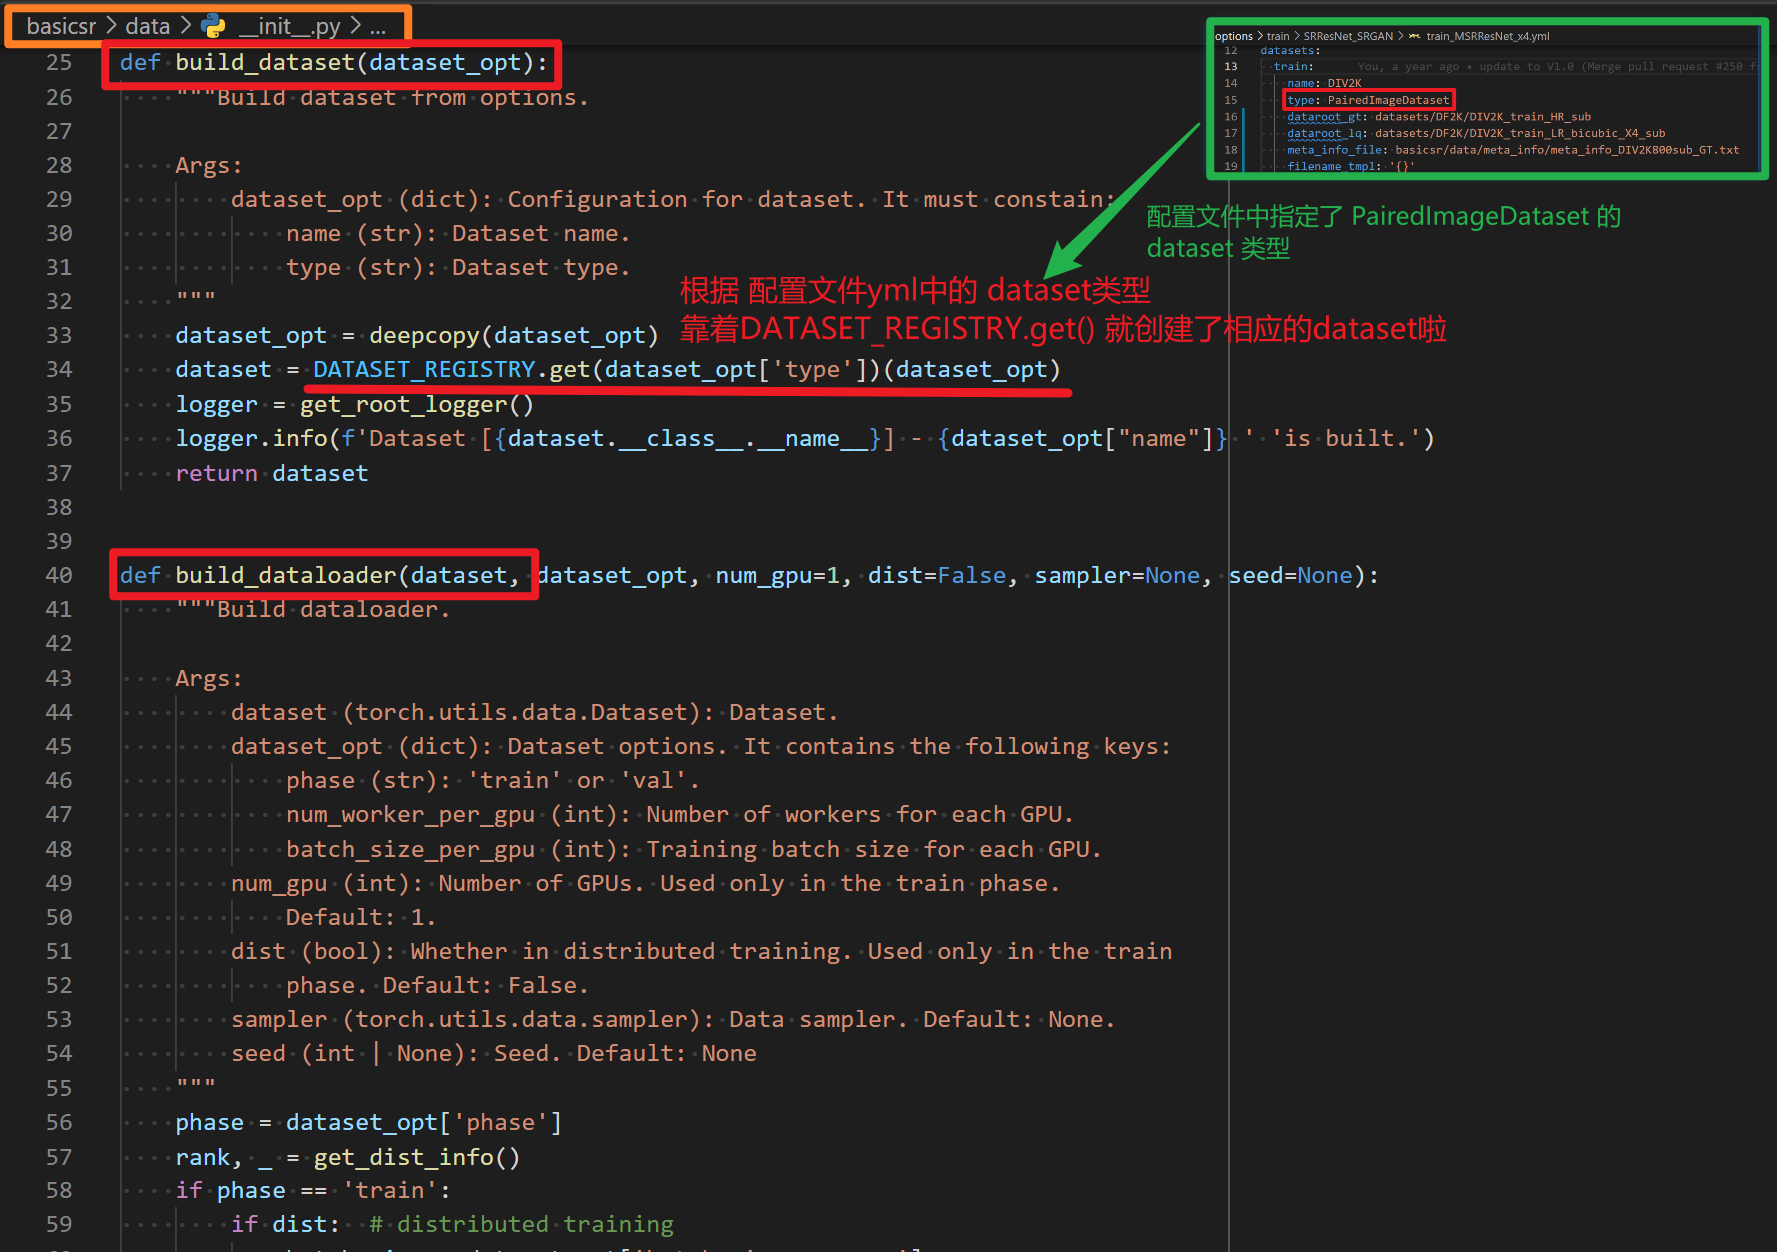
\includegraphics[width=0.7\linewidth]{figures/getting_start_10.png}
                  \caption{定义 build\_dataloader 和 build\_dataset }
                  \label{fig:getting_start_10}
              \end{center}
              \vspace{-0.5cm}
          \end{figure}

          build\_dataset 是核心。在这里,它会根据配置文件 yml 中的 dataset 类型,比如在我们这个例子中就是 PairedImageDataset ,创建相应的实例。核心就一句代码:DATASET\_REGISTRY.get() 。关于这块具体是如何做到根据“类名”动态创建实例的,我们会在下一篇文章中讲解它的机制。(实例就是由类 class 创建的,具体运行的对象)。这里我们只要理解,通过这一句调用,就可以创建相应的实例了。
          build\_dataloader 是比较容易理解的。它根据传入的 dataset 和其他在 yml 中的参数,构建 dataloader。

    \item model 的创建
          model 的创建是通过 build\_model 这个函数,定义在 basicsr/models/\_\_init\_\_.py 文件里面。

          \begin{figure}[H]
              \begin{center}
                  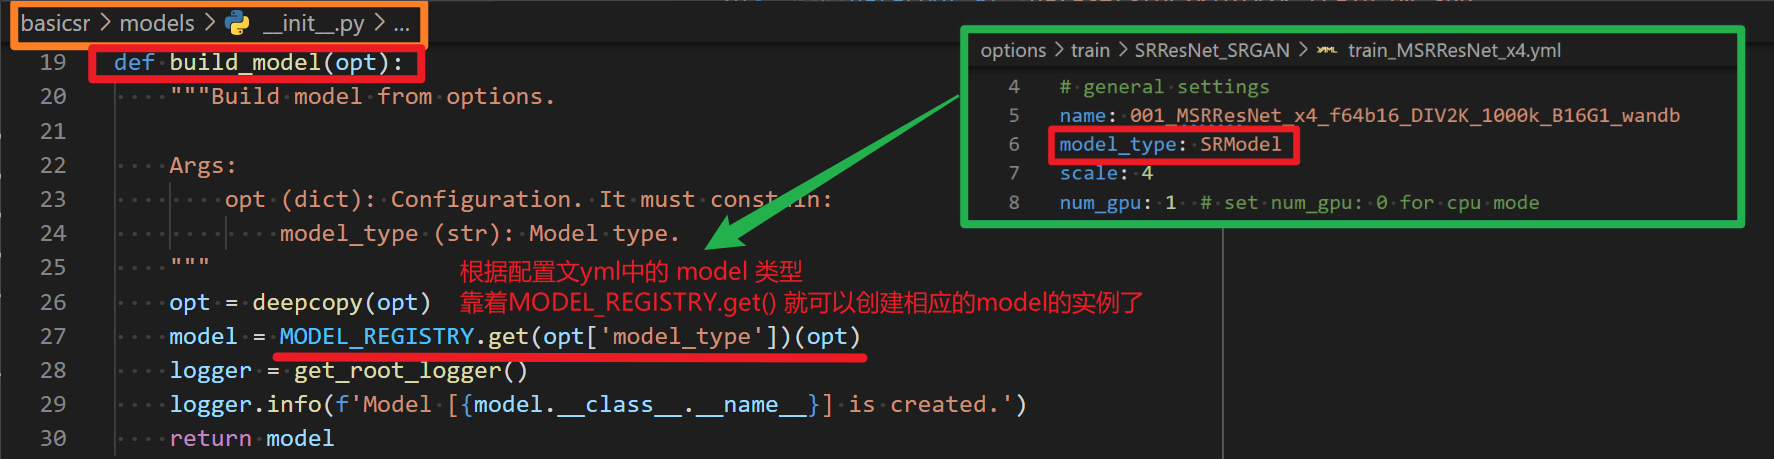
\includegraphics[width=0.7\linewidth]{figures/getting_start_11.png}
                  \caption{基于 build\_model 定义 model 的类型}
                  \label{fig:getting_start_11}
              \end{center}
              \vspace{-0.5cm}
          \end{figure}

          build\_model 会根据配置文件 yml 中的 model 类型,比如在我们这个例子中就是 SRModel ,创建相应的实例。
          额外说一句,在 BasicSR 框架中,主要有以下几个类型,都是通过 REGISTRY 的机制来方便地实例化的:

          \begin{figure}[H]
              \begin{center}
                  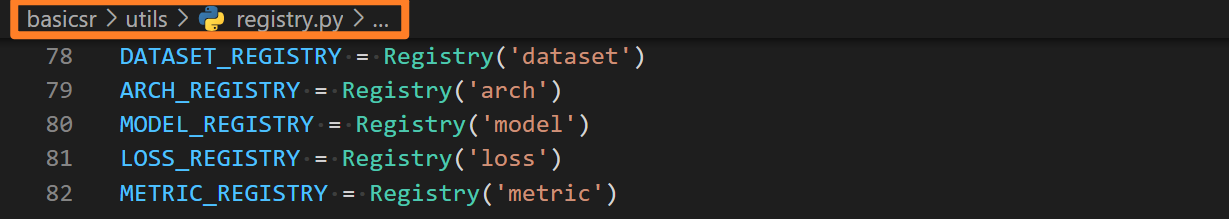
\includegraphics[width=0.7\linewidth]{figures/getting_start_12.png}
                  \caption{基于 REGISTRY 进行实例化}
                  \label{fig:getting_start_12}
              \end{center}
              \vspace{-0.5cm}
          \end{figure}

          接下来我们再具体地看看 SRModel 这个实例的创建过程吧,以便更好地理解一个模型中做了什么操作。
          让我们进入 SRModel 这个类。

          \begin{figure}[H]
              \begin{center}
                  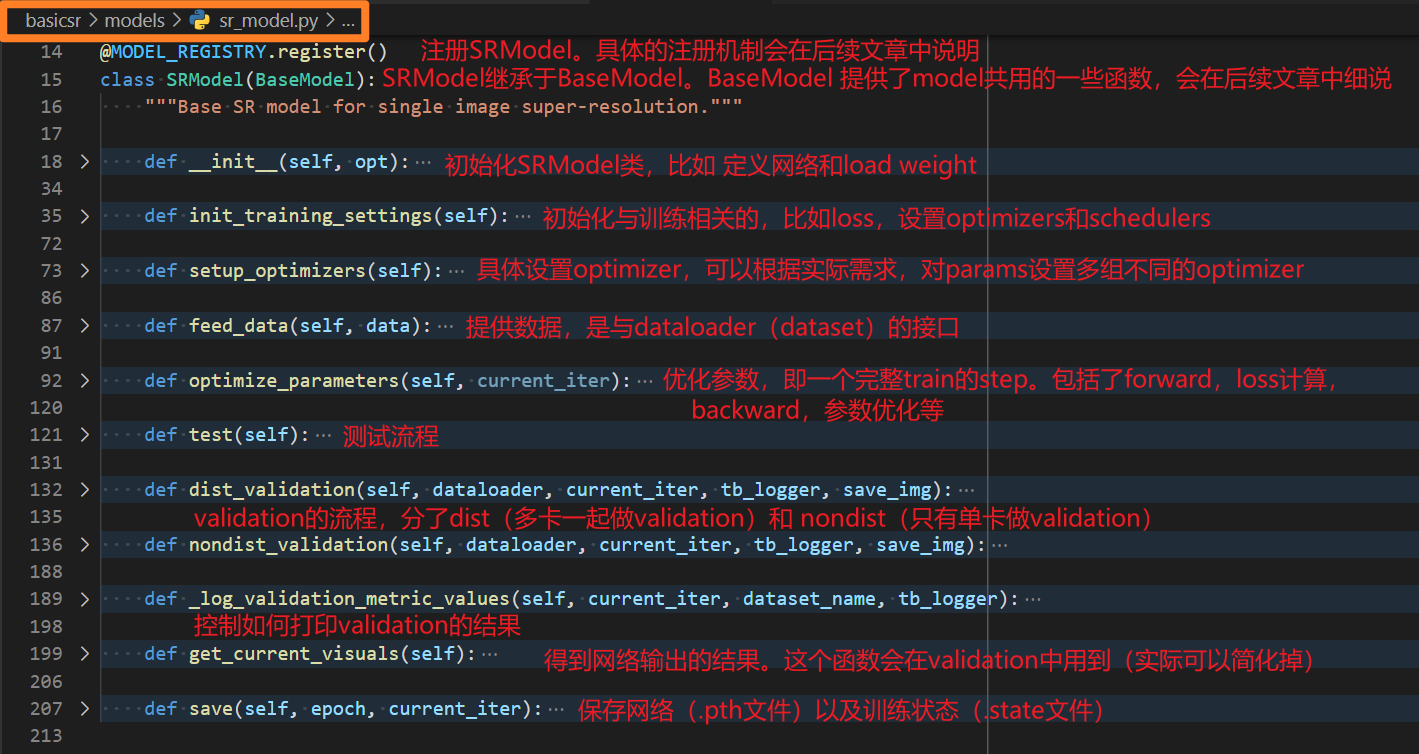
\includegraphics[width=0.7\linewidth]{figures/getting_start_13.png}
                  \caption{SR model 类的定义}
                  \label{fig:getting_start_13}
              \end{center}
              \vspace{-0.5cm}
          \end{figure}

          在这个章节的介绍中,我们主要关注以下几个方面:

          \begin{enumerate}
              \item network 的创建
              \item loss 的创建
              \item optimize\_parameters ,即一个 iteration 的 train step
              \item metric 的使用
          \end{enumerate}

          下面我们分别简略说明,希望大家可以抓住大致的脉络。

          \begin{enumerate}

              \item network 的创建一般是在 model 的 \_\_init\_\_() 函数里面,是通过调用 build\_network() 实现的。 \_\_init\_\_() 函数一般还会加载预训练模型,并初始化训练相关的设置。

                    \begin{figure}[H]
                        \begin{center}
                            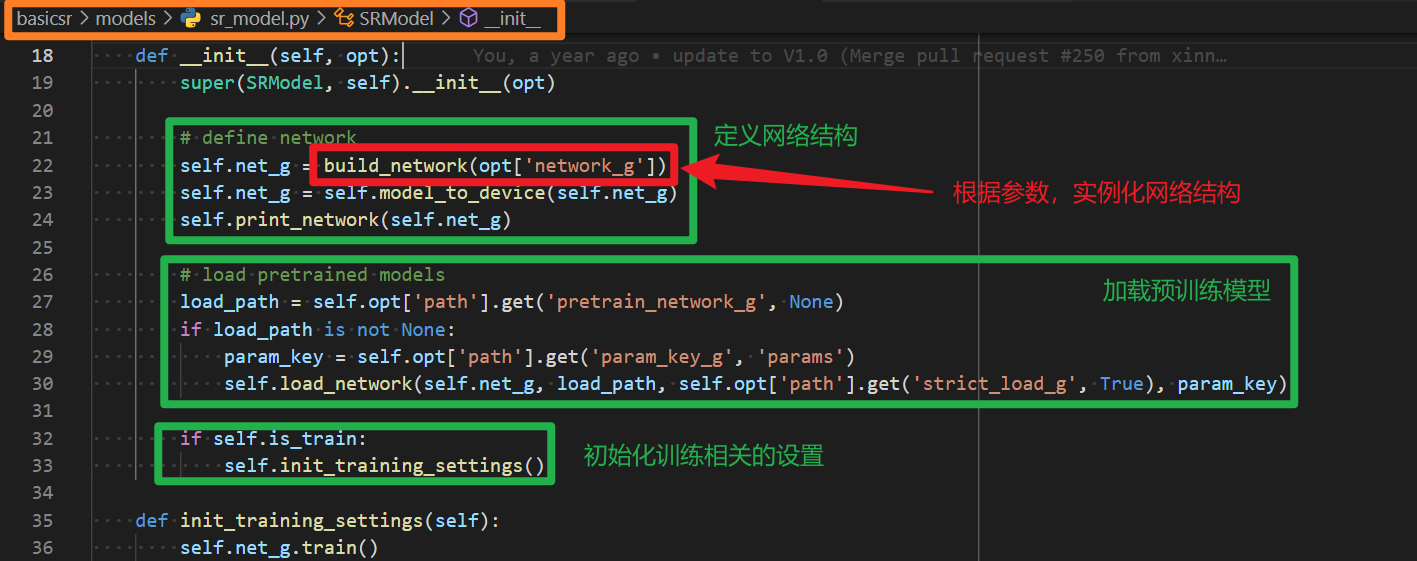
\includegraphics[width=0.7\linewidth]{figures/getting_start_14.png}
                            \caption{定义网络结构}
                            \label{fig:getting_start_14}
                        \end{center}
                        \vspace{-0.5cm}
                    \end{figure}

                    build\_network 会根据配置文件 yml 中的 network 类型,比如在我们这个例子中就是 MSRResNet ,创建相应的实例。使用的是 ARCH\_REGISTRY 。

                    \begin{figure}[H]
                        \begin{center}
                            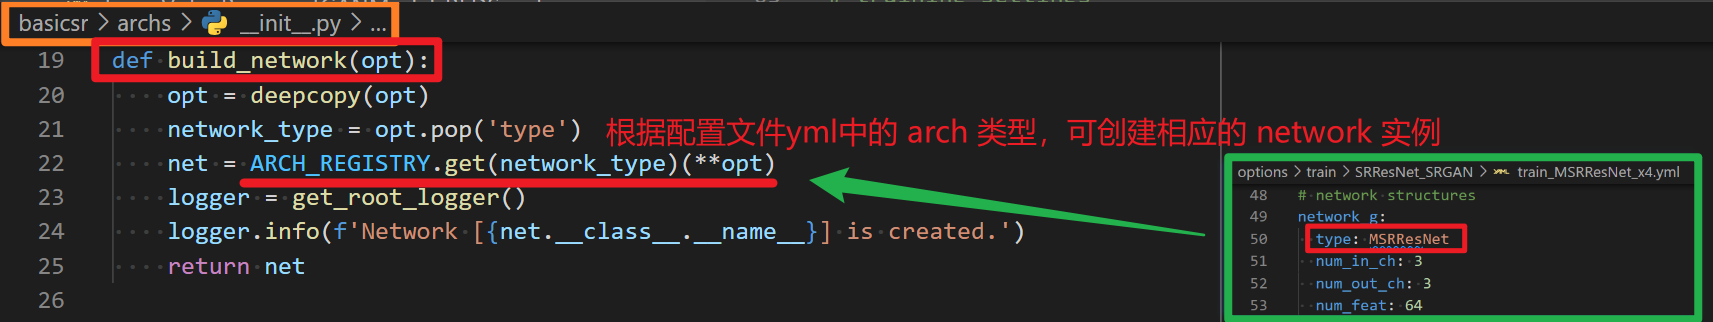
\includegraphics[width=0.7\linewidth]{figures/getting_start_15.png}
                            \caption{基于 yml 文件配置创建 network 实例}
                            \label{fig:getting_start_15}
                        \end{center}
                        \vspace{-0.5cm}
                    \end{figure}

              \item loss 的创建一般是在 model 的 init\_training\_settings() 函数里面。其他可以不用太关注,我们主要关注 build\_loss 这个函数。loss 就是通过调用 build\_loss() 实现的。如果有多个 loss ,则会多次调用 build\_loss() ,创建多个 loss 实例。

                    \begin{figure}[H]
                        \begin{center}
                            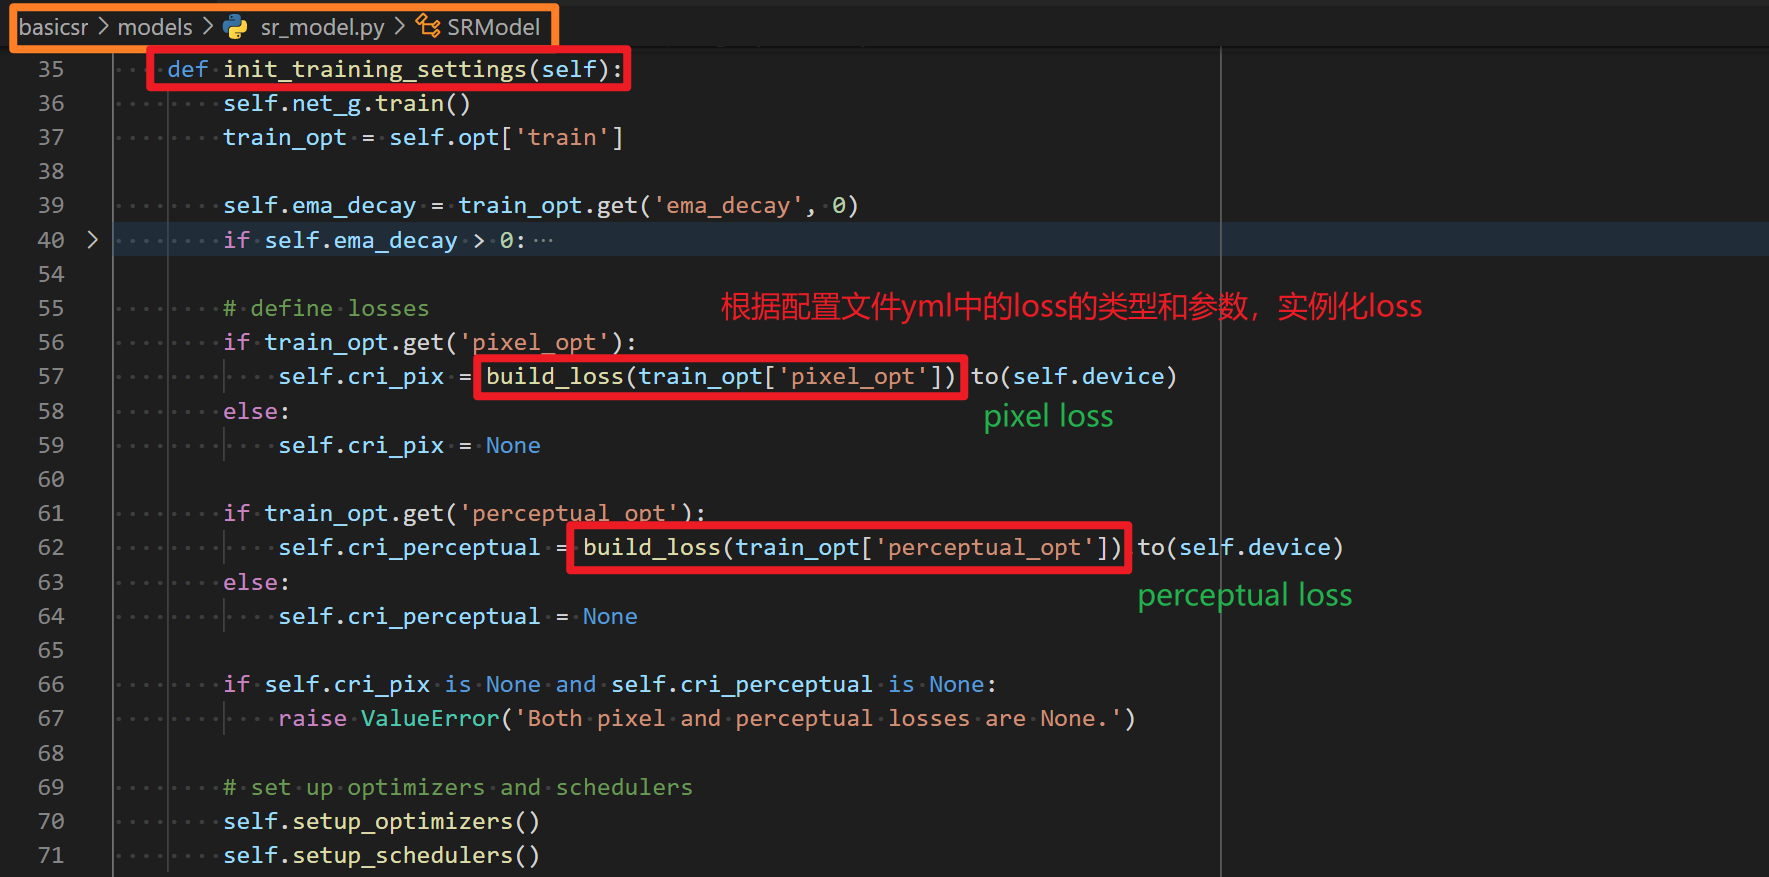
\includegraphics[width=0.7\linewidth]{figures/getting_start_16.png}
                            \caption{基于 yml 文件配置创建 loss 实例}
                            \label{fig:getting_start_16}
                        \end{center}
                        \vspace{-0.5cm}
                    \end{figure}

                    build\_loss 会根据配置文件 yml 中的 loss 类型,比如在我们这个例子中就是 L1Loss ,创建相应的实例。使用的是  LOSS\_REGISTRY 。

                    \begin{figure}[H]
                        \begin{center}
                            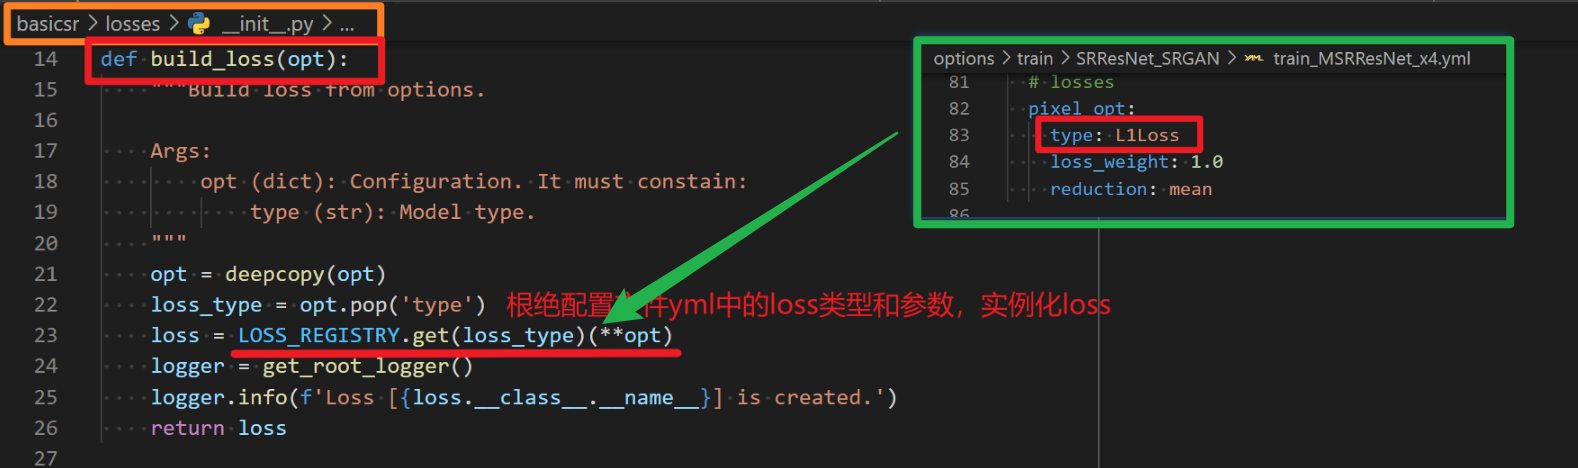
\includegraphics[width=0.7\linewidth]{figures/getting_start_17.png}
                            \caption{基于 yml 文件 L1 loss 配置创建 L1 loss 实例}
                            \label{fig:getting_start_17}
                        \end{center}
                        \vspace{-0.5cm}
                    \end{figure}

              \item optimize\_parameters,即一个 iteration 下的 train step 。这个函数里面主要包含了 network forward ,loss 计算,backward 和优化器的更新。

                    \begin{figure}[H]
                        \begin{center}
                            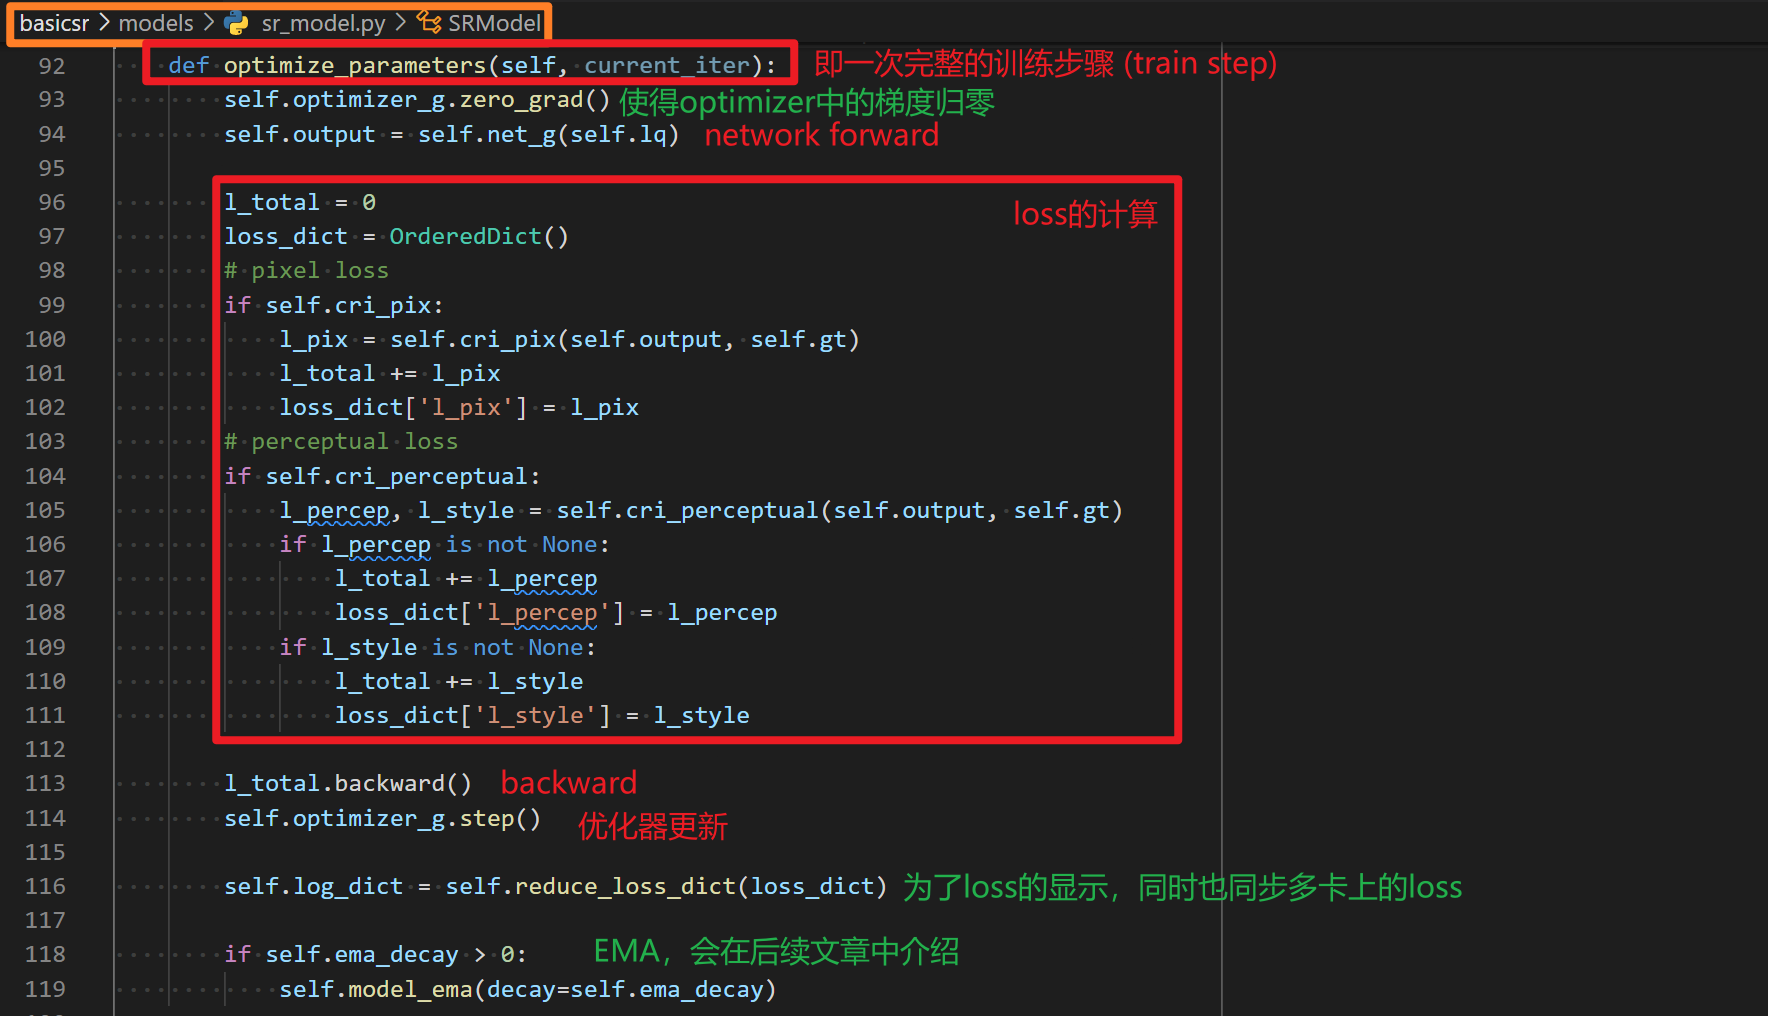
\includegraphics[width=0.7\linewidth]{figures/getting_start_18.png}
                            \caption{一个 iteration 的参数优化过程}
                            \label{fig:getting_start_18}
                        \end{center}
                        \vspace{-0.5cm}
                    \end{figure}

              \item metric 的使用主要是在 validation 里面。我们来看在训练 MSRResNet 中调用的 nondist\_validation 函数。其中核心是在 calculate\_metric 这个函数,它会根据配置文件 yml 中的 metrics 配置,调用相应的函数

                    \begin{figure}[H]
                        \begin{center}
                            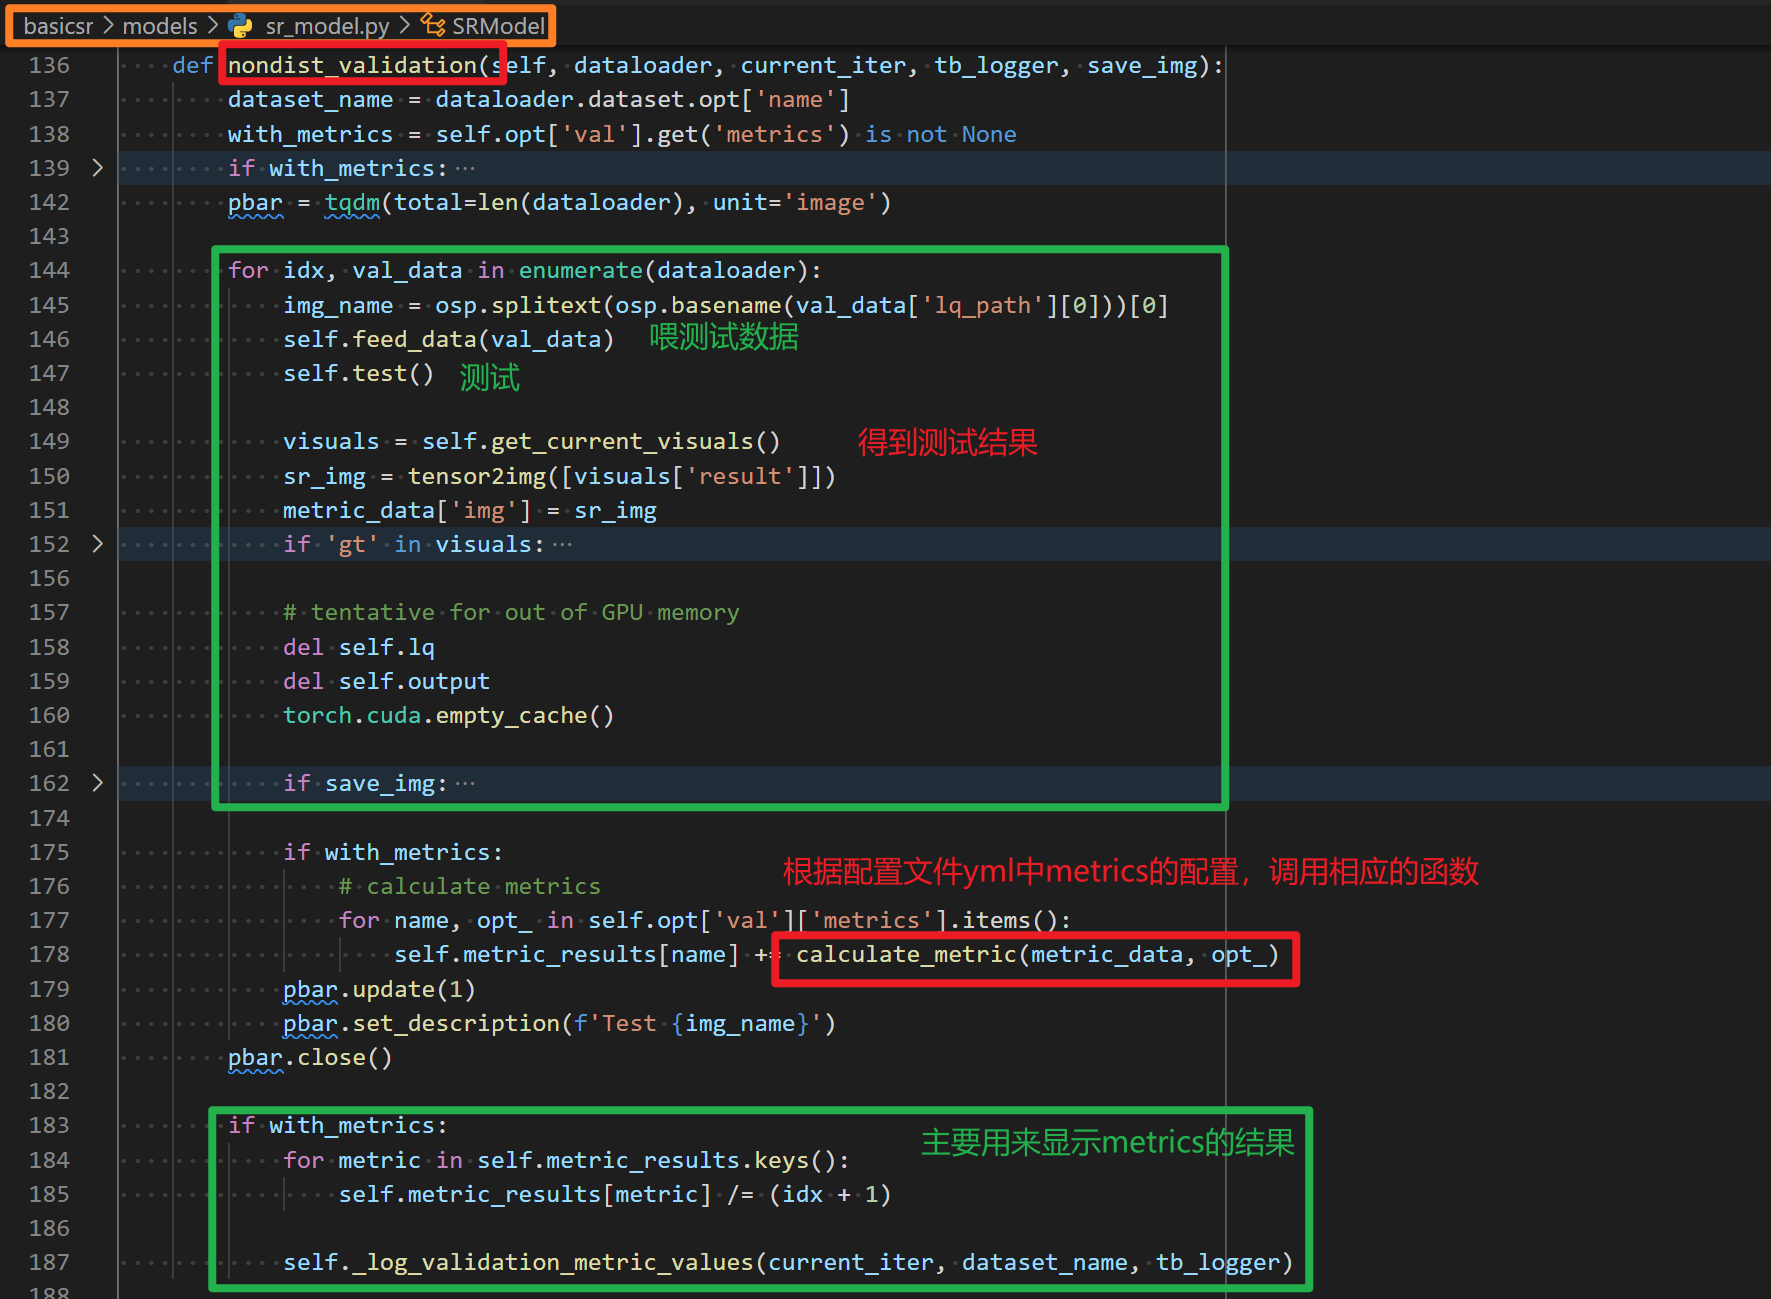
\includegraphics[width=0.7\linewidth]{figures/getting_start_19.png}
                            \caption{基于 yml 文件配置调用对应的 metric 函数}
                            \label{fig:getting_start_19}
                        \end{center}
                        \vspace{-0.5cm}
                    \end{figure}

                    calculate\_metric 具体定义在 basicsr/metrics/\_\_init\_\_() 文件中,它也是使用了 REGISTRY 机制 ——METRIC\_REGISTRY。它会根据配置文件 yml 中的 metric 类型,比如在我们这个例子中就是有两个 metrics:PSNR 和 SSIM ,调用相应的函数。注意和前面 DATASET, ARCH, MODEL, LOSS 的 REGISTRY 不同,这里返回的是函数调用,而其他返回的是类的实例。
                    \begin{figure}[H]
                        \begin{center}
                            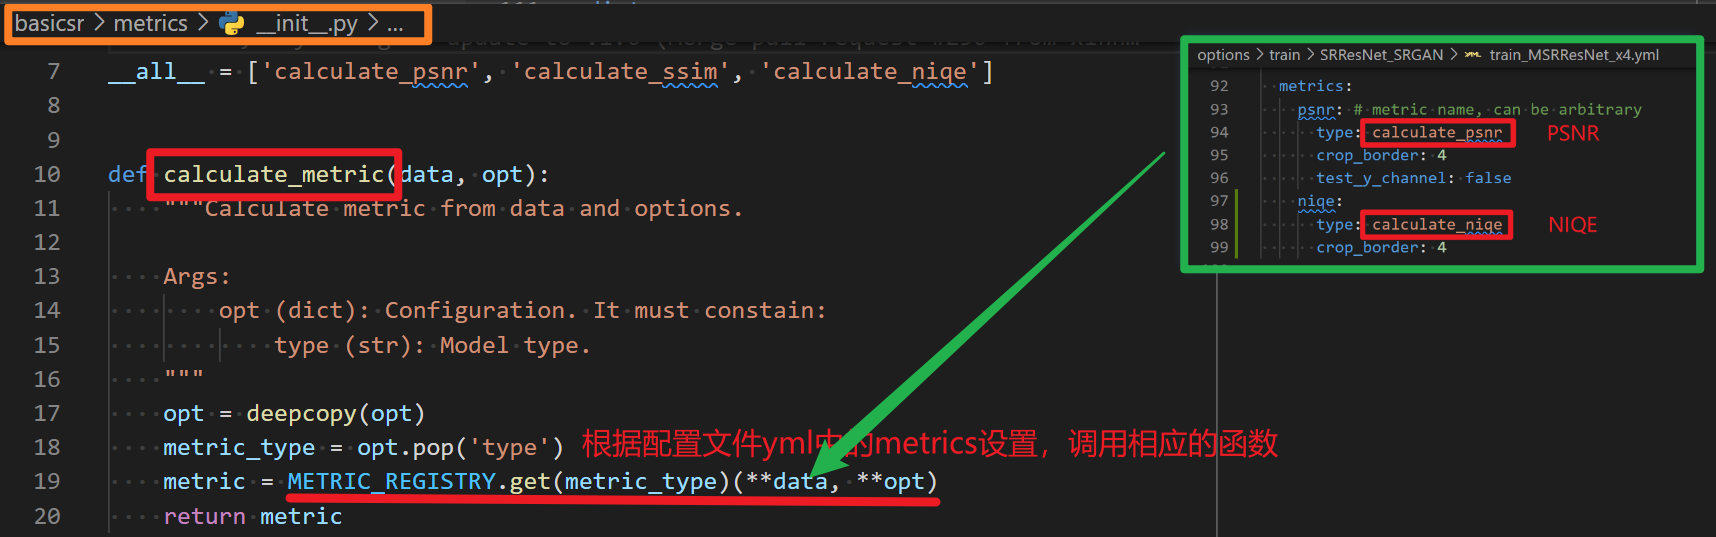
\includegraphics[width=0.7\linewidth]{figures/getting_start_20.png}
                            \caption{基于 yml 文件配置调用 PSNR 和 SSIM 函数}
                            \label{fig:getting_start_19}
                        \end{center}
                        \vspace{-0.5cm}
                    \end{figure}

                    到此,我们已经看到了 data 的创建,以及 model 的创建。model 的创建包含了 network architecture 和 loss 的创建,一次完整的训练流程以及 validation 中用到的 metric 的计算。

          \end{enumerate}

          % ----------------------------------
          \subsection{训练过程}

          最后一块就是训练过程了。它就是一个循环的过程,不断地喂数据,然后不断执行训练步骤。整个训练过程如下,看图就可以啦,不用多说啦。

          \begin{figure}[H]
              \begin{center}
                  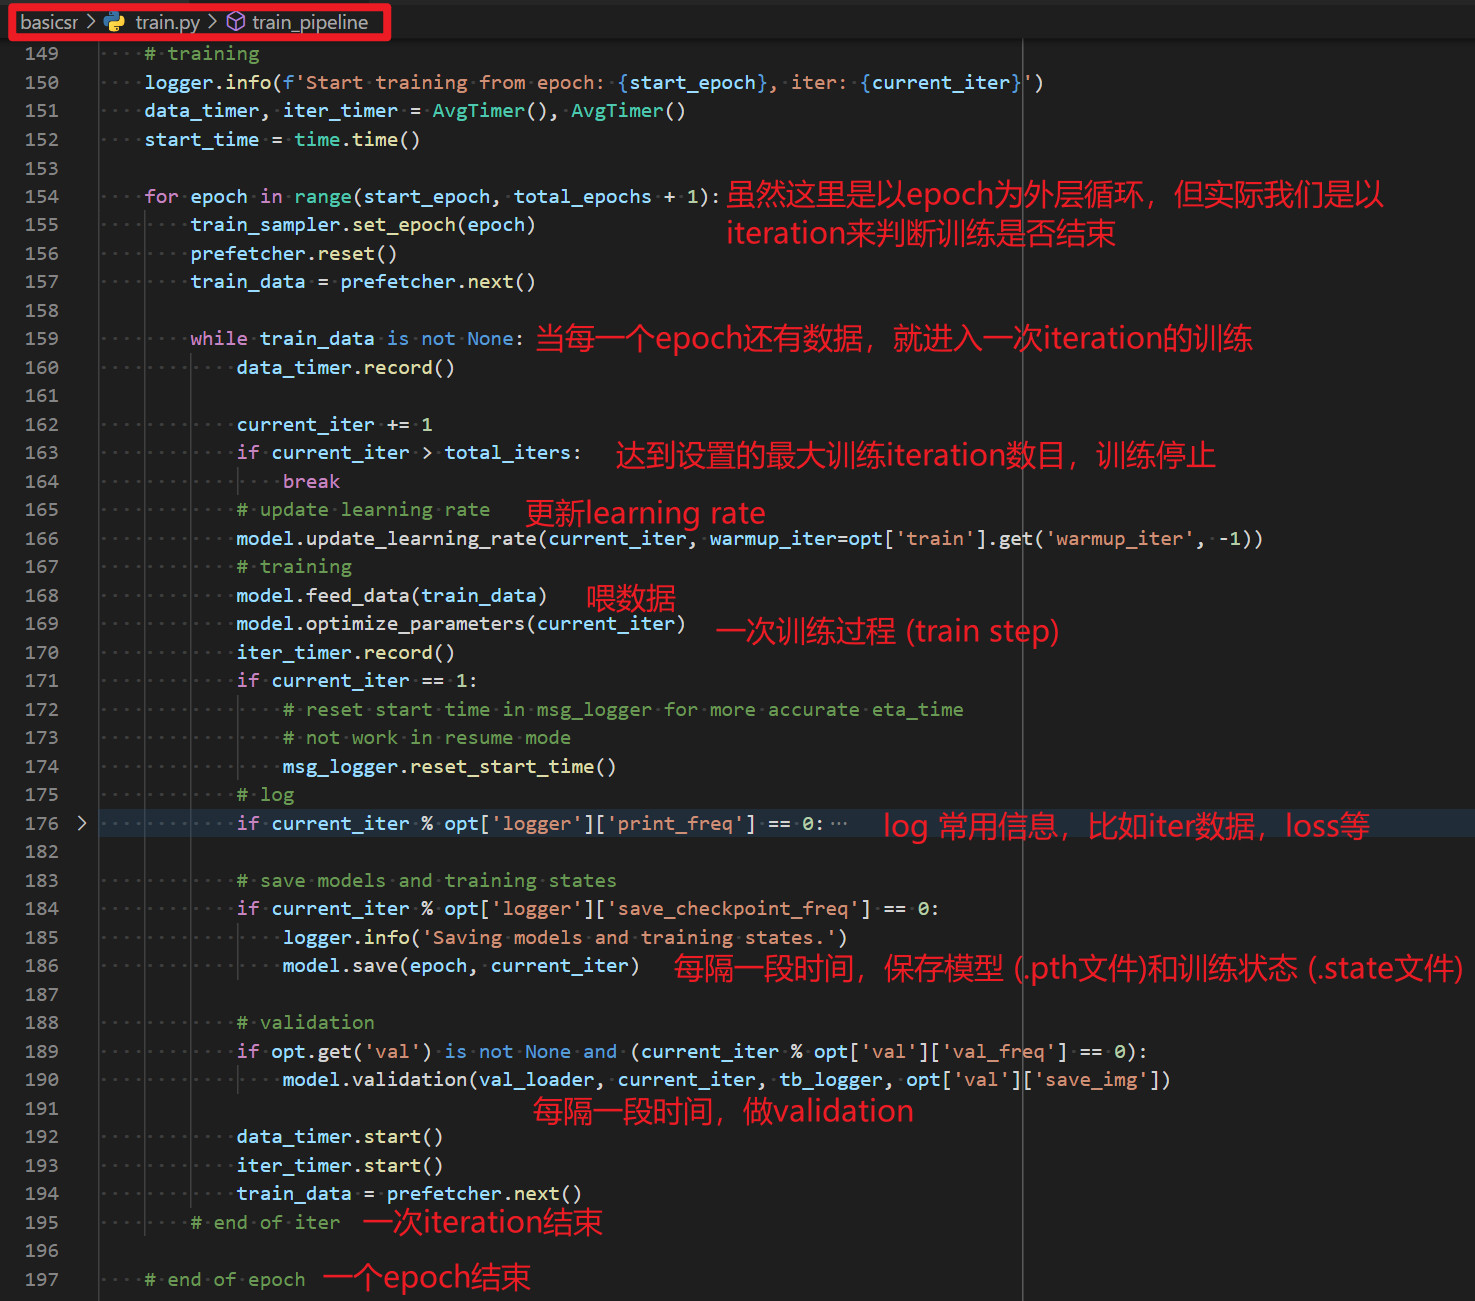
\includegraphics[width=0.7\linewidth]{figures/getting_start_21.png}
                  \caption{完整的训练过程}
                  \label{fig:getting_start_19}
              \end{center}
              \vspace{-0.5cm}
          \end{figure}

          上面的 for 循环结束,整个训练过程也就结束啦。










          %     其中 train\_MSRResNet\_x4.yml 为 yml 配置文件,设置所有与实验相关的配置参数。

          %     对于一些大型模型,可能需要采用分布式来进行训练,相关的命令可参考:
          %     \href{https://github.com/XPixelGroup/BasicSR/blob/master/docs/TrainTest.md}{分布式训练和测试命令}

          %     \item 在训练的命令行中,可以采用一些参数来进行训练对配置

          %     \begin{enumerate}
          %     \item \textbf{$-$opt}:配置文件的路径。
          %     \item \textbf{$--$laucher}:用于指定分布式训练,比如pytorch或者slurm。默认是none,即单卡非distributed training。
          %     \item \textbf{$--$auto\_resume}:自动查找最近的checkpoint继续训练。程序异常中断,在命令行中添加这个参数,就可以实现自动resume。
          %     \item \textbf{$--$debug}:能够快速帮助debug。进入debug模式后,每个iter都会print log,8个iter后就会validation。这样可以快速方便地查看代码是否可以正常运行。
          %     \item \textbf{$--$local\_rank}:分布式训练程序自动会传入
          %     \item \textbf{$--$force\_yml}:在命令行中修改yml中的配置文件。一般不推荐使用,除非你非常清楚自己所做的事。
          %     \end{enumerate}

          % \item 训练文件

          % 输入指令后,BasicSR/basicsr/train.py文件中的代码就开始执行训练
          % \begin{minted}[xleftmargin=20pt,linenos,bgcolor=bg]{python}
          % if __name__ == '__main__':
          %     root_path = osp.abspath(osp.join(__file__, osp.pardir, osp.pardir))
          %     train_pipeline(root_path)
          % \end{minted}
          % 首先需要把root\_path作为参数传进去,当我们把basicsr作为package使用的时候,需要根据当前的目录路径来创建文件,否则程序会错误地使用basicsr package所在位置的目录了。

          % 其中,train\_pipeline函数的流程主要为主要有:
          % \begin{enumerate}

          % \item 初始化定义

          % \begin{minted}[xleftmargin=20pt,linenos,breaklines,bgcolor=bg]{python}
          % def train_pipeline(root_path):
          %     opt, args = parse_options(root_path, is_train=True)
          %     opt['root_path'] = root_path
          % # 解析yml配置文件和其他配置操作,比如分布式训练和随机种子等
          %     torch.backends.cudnn.benchmark = True
          %     resume_state = load_resume_state(opt)
          % # 如果有resume指令,则会加载设置的.stat文件
          %     if resume_state is None:
          %         make_exp_dirs(opt)
          %         if opt['logger'].get('use_tb_logger') and 'debug'
          %         not in opt['name'] and opt['rank'] == 0:
          %             mkdir_and_rename(osp.join(opt['root_path'],
          %             'tb_logger', opt['name']))
          % # 创建实验所需文件夹,如果有resume则不需要创建
          %     copy_opt_file(args.opt, opt['path']['experiments_root'])
          % # 注意在这以上代码(及函数调用)中,不能使用get\_root\_logger,
          % # 否则会导致logger初始化错误
          %     log_file = osp.join(opt['path']['log'],
          %     f"train_{opt['name']}_{get_time_str()}.log")
          %     logger = get_root_logger(logger_name='basicsr', log_level=logging.INFO,
          %     log_file=log_file)
          %     logger.info(get_env_info())
          % # 初始化日志系统logger,生成文件和屏幕的logger显示
          %     logger.info(dict2str(opt))
          % # 输出环境和配置信息
          %     tb_logger = init_tb_loggers(opt)
          % # 根据配置需要,初始化tensorboard和wandb的logger

          % \end{minted}
          % \end{enumerate}

          % \subsection{Data 和 Model 的创建}


          % \begin{enumerate}

          % \item 数据和模型等的初始化

          % \begin{minted}[xleftmargin=20pt,linenos,breaklines,bgcolor=bg]{python}
          % # 创建训练和验证的dataloaders
          % result = create_train_val_dataloader(opt, logger)
          % train_loader, train_sampler, val_loaders, total_epochs, total_iters = result
          % # 创建模型
          % model = build_model(opt)
          % if resume_state:  # resume training
          %     model.resume_training(resume_state)  # handle optimizers and schedulers
          %     logger.info(f"Resuming training from epoch: {resume_state['epoch']},
          %     iter: {resume_state['iter']}.")
          %     start_epoch = resume_state['epoch']
          %     current_iter = resume_state['iter']
          % else:
          %     start_epoch = 0
          %     current_iter = 0
          % # 创建实验信息的logger来输出
          % msg_logger = MessageLogger(opt, current_iter, tb_logger)
          % # dataloader prefetcher
          % prefetch_mode = opt['datasets']['train'].get('prefetch_mode')
          % if prefetch_mode is None or prefetch_mode == 'cpu':
          %     prefetcher = CPUPrefetcher(train_loader)
          % elif prefetch_mode == 'cuda':
          %     prefetcher = CUDAPrefetcher(train_loader, opt)
          %     logger.info(f'Use {prefetch_mode} prefetch dataloader')
          %     if opt['datasets']['train'].get('pin_memory') is not True:
          %         raise ValueError('Please set pin_memory=True for CUDAPrefetcher.')
          % else:
          %     raise ValueError(f"Wrong prefetch_mode {prefetch_mode}.
          %     Supported ones are: None, 'cuda', 'cpu'.")

          % \end{minted}
          % \end{enumerate}

          % \subsection{训练过程}

          % \begin{enumerate}
          % \item 训练流程
          % 本小节是训练过程中对主要代码块,在经过了训练参数的初始化,数据和模型的初始化了之后,程序就从start\_epoch开始训练只至total\_epochs+1训练结束。其中主要的功能逻辑流为:

          % \begin{enumerate}
          % \item 更新学习率
          % \item 加载数据
          % \item 执行一次训练,更新网络参数
          % \item 保存日志信息
          % \item 达到预设迭代次数,执行验证或者保存模型
          % \end{enumerate}

          % \begin{minted}[xleftmargin=20pt,linenos,breaklines,bgcolor=bg]{python}
          % # line149 - 200
          % logger.info(f'Start training from epoch: {start_epoch}, iter: {current_iter}')
          % data_timer, iter_timer = AvgTimer(), AvgTimer()
          % start_time = time.time()

          % for epoch in range(start_epoch, total_epochs + 1):
          %     train_sampler.set_epoch(epoch)
          %     prefetcher.reset()
          %     train_data = prefetcher.next()
          % # 以epoch为外层循环,但是在yml配置文件中使用的是iteration来进行设置
          %     while train_data is not None:
          % # 当每一个epoch还有数据,就进入一次iteration的训练
          %         data_timer.record()
          %         current_iter += 1
          %         if current_iter > total_iters:
          %             break
          % # 达到设置的最大训练iteration数目,训练停止
          %         model.update_learning_rate(current_iter,
          %         warmup_iter=opt['train'].get('warmup_iter', -1))
          % # 更新学习率
          %         model.feed_data(train_data)
          % # 加入数据
          %         model.optimize_parameters(current_iter)
          % # 执行一次训练
          %         iter_timer.record()
          %         if current_iter == 1:
          %             # 重新设置msg_logger的开始时间
          %             # resume 模式下不启用
          %             msg_logger.reset_start_time()
          %         # log 文件设置
          %         if current_iter % opt['logger']['print_freq'] == 0:
          %             log_vars = {'epoch': epoch, 'iter': current_iter}
          %             log_vars.update({'lrs': model.get_current_learning_rate()})
          %             log_vars.update({'time': iter_timer.get_avg_time(),
          %             'data_time': data_timer.get_avg_time()})
          %             log_vars.update(model.get_current_log())
          %             msg_logger(log_vars)
          % # 保存训练的实验参数,比如loss等
          %         if current_iter % opt['logger']['save_checkpoint_freq'] == 0:
          %             logger.info('Saving models and training states.')
          %             model.save(epoch, current_iter)
          % # 根据yml设置的参数,每隔一段时间保存模型(.pth)和训练状态文件(.state)
          %         # validation
          %         if opt.get('val') is not None and (current_iter
          %             if len(val_loaders) > 1:
          %                 logger.warning('Multiple validation datasets are
          %                 *only* supported by SRModel.')
          %             for val_loader in val_loaders:
          %                 model.validation(val_loader, current_iter,
          %                 tb_logger, opt['val']['save_img'])
          % # 根据yml设置的参数,进行一次validation
          %         data_timer.start()
          %         iter_timer.start()
          %         train_data = prefetcher.next()
          %     # 结束一个iteration
          % # 结束一个epoch
          % \end{minted}

          % \end{enumerate}

          % % 4. 相关的函数定义

          % % \begin{enumerate}
          % % \item build\_dataset和build\_dataloader
          % % \item build\_model
          % % \end{enumerate}

          % \end{enumerate}


          % \section{测试流程}


          % 测试阶段,我们需要在终端输入命令来开始训练。
          % \begin{minted}[xleftmargin=20pt,linenos,breaklines,bgcolor=bg]{python}
          % CUDA_VISIBLE_DEVICES=0 python basicsr/test.py -opt options/test/SRResNet_SRGAN/test_MSRResNet_x4.yml
          % \end{minted}

          % 其中test\_MSRResNet\_x4为yml配置文件,主要设置实验相关的超参数和相关的一些配置参数。

          % \begin{hl} % ---------------- Highlight block ---------------- %

          %     \textbf{测试注意事项}

          %     如果需要额外添加测试集,需要使用test\_x格式,下划线之后是测试集的编号

          %     路径需要设置为待测模型所在的路径

          %     suffix配置为存储图片的名字后缀,一般设置为这个方法的名字便于对比

          %     metrics里面设置需要的评价指标,PSNR,SSIM和NIQE等

          %     分布式测试命令可参考:
          % \href{https://github.com/XPixelGroup/BasicSR/blob/master/docs/TrainTest.md}{分布式训练和测试命令}

          % \end{hl}





          % \begin{minted}[xleftmargin=20pt,linenos,bgcolor=bg]{python}

          % def test_pipeline(root_path):
          %     # 加载配置参数
          %     opt, _ = parse_options(root_path, is_train=False)
          %     torch.backends.cudnn.benchmark = True

          %     # 新建loggers并初始化
          %     make_exp_dirs(opt)
          %     log_file = osp.join(opt['path']['log'],
          %     f"test_{opt['name']}_{get_time_str()}.log")
          %     logger = get_root_logger(logger_name='basicsr',
          %     log_level=logging.INFO, log_file=log_file)
          %     logger.info(get_env_info())
          %     logger.info(dict2str(opt))

          %     # 创建测试集和dataloader
          %     test_loaders = []
          %     for _, dataset_opt in sorted(opt['datasets'].items()):
          %         test_set = build_dataset(dataset_opt)
          %         test_loader = build_dataloader(
          %             test_set, dataset_opt, num_gpu=opt['num_gpu'],
          %             dist=opt['dist'], sampler=None, seed=opt['manual_seed'])
          %         logger.info(f"Number of test images in {dataset_opt['name']}:
          %         {len(test_set)}")
          %         test_loaders.append(test_loader)

          %     # 创建模型
          %     model = build_model(opt)
          %     # 测试多个测试集
          %     for test_loader in test_loaders:
          %         test_set_name = test_loader.dataset.opt['name']
          %         logger.info(f'Testing {test_set_name}...')
          %         model.validation(test_loader, current_iter=opt['name'],
          %         tb_logger=None, save_img=opt['val']['save_img'])


          % if __name__ == '__main__':
          %     root_path = osp.abspath(osp.join(__file__, osp.pardir, osp.pardir))
          %     test_pipeline(root_path)
          % \end{minted}


          % \section{推理流程}

          % 快速推理阶段,我们需要在终端输入命令来进行快速推理:
          % \begin{minted}[xleftmargin=20pt,linenos,breaklines,bgcolor=bg]{python}
          % CUDA_VISIBLE_DEVICES=0 python basicsr/inference/inference_esrgan.py --input input_path --output out_path
          % \end{minted}

          % \begin{hl} % ---------------- Highlight block ---------------- %

          %     \textbf{推理注意事项}

          %     需要提前下载好预训练模型放在experiments/pretrained\_models/ 下面,在配置参数中可以详细的对比下载存放的路径和代码中设置的路径

          %     和测试不同,快速推理不涉及到定量评价指标的计算,比如PSNR,SSIM和NIQE等

          %     分布式测试命令可参考:
          % \href{https://github.com/XPixelGroup/BasicSR/blob/master/docs/TrainTest.md}{分布式训练和测试命令}

          % \end{hl}



          % \begin{minted}[xleftmargin=20pt,linenos,breaklines,bgcolor=bg]{python}

          % #加载配置参数
          % parser = argparse.ArgumentParser()
          % parser.add_argument(
          %     '--model_path',
          %     type=str,
          %     default=  # noqa: E251
          %     'experiments/pretrained_models/ESRGAN/
          %     ESRGAN_SRx4_DF2KOST_official-ff704c30.pth'  # noqa: E501
          % )
          % parser.add_argument('--input', type=str,
          % default='datasets/Set14/LRbicx4', help='input test image folder')
          % parser.add_argument('--output', type=str, default='results/ESRGAN',
          % help='output folder')
          % args = parser.parse_args()

          % device = torch.device('cuda' if torch.cuda.is_available() else 'cpu')
          % # 设置快速推理所需要模型
          % model = RRDBNet(num_in_ch=3, num_out_ch=3, num_feat=64,
          % num_block=23, num_grow_ch=32)
          % model.load_state_dict(torch.load(args.model_path)['params'], strict=True)
          % model.eval()
          % model = model.to(device)

          % # 设置快速推理后输出的存放路径
          % os.makedirs(args.output, exist_ok=True)
          % for idx, path in enumerate(sorted(glob.glob(os.path.join(args.input, '*')))):
          %     imgname = os.path.splitext(os.path.basename(path))[0]
          %     print('Testing', idx, imgname)
          %     # 读取图片
          %     img = cv2.imread(path, cv2.IMREAD_COLOR).astype(np.float32) / 255.
          %     img = torch.from_numpy(np.transpose(img[:, :, [2, 1, 0]], (2, 0, 1))).float()
          %     img = img.unsqueeze(0).to(device)
          %     # 快速推理
          %     try:
          %         with torch.no_grad():
          %             output = model(img)
          %     except Exception as error:
          %         print('Error', error, imgname)
          %     else:
          %         # 保存图片
          %         output = output.data.squeeze().float().cpu().clamp_(0, 1).numpy()
          %         output = np.transpose(output[[2, 1, 0], :, :], (1, 2, 0))
          %         output = (output * 255.0).round().astype(np.uint8)
          %         cv2.imwrite(os.path.join(args.output, f'{imgname}_ESRGAN.png'), output)
          % \end{minted}

          % \section{入门样例}

          % 这个部分我们以一个基础的超分模型SRResNet作为例子来展示BasicSR的入门使用。相关的文件目录如下所示:

          % \dirtree{%
          %     .1 \textcolor{black}{BasicSR}.
          %     .2 \textcolor{red}{basicsr}\DTcomment{BasicSR核心代码包}.
          %     .2 scripts\DTcomment{常用脚本}.
          %     .3 data\_preparation\DTcomment{数据准备脚本目录}.
          %     .4 extract\_subimages.py\DTcomment{生成子图脚本}.
          %     .2 datasets\DTcomment{数据集存放,推荐soft link}.
          %     .3 DIV2K\DTcomment{训练数据集}.
          %     .4 DIV2K\_train\_HR\_sub\DTcomment{训练数据集的GT子图}.
          %     .4 DIV2K\_train\_LR\_bicubic\_X4\_sub\DTcomment{训练数据集子图的下采样图}.
          %     .3 Set5\DTcomment{验证集}.
          %     .4 GTmod12\DTcomment{验证集的GT图}.
          %     .4 LRbicx4\DTcomment{验证集的下采样图}.
          %     .3 Set14\DTcomment{验证集}.
          %     .4 GTmod12\DTcomment{验证集的GT图}.
          %     .4 LRbicx4\DTcomment{验证集的下采样图}.
          %     .2 experiments\DTcomment{实验保存路径}.
          %     .3 pretrained\_models\DTcomment{预训练模型保存路径}.
          %     .3 001\_MSRResNet\_x4\_f64b16\_DIV2K\_1000k\_B16G1\_wandb\DTcomment{SRResNet实验存放路径}.
          %     .4 models\DTcomment{SRResNet训练模型存放位置}.
          %     .4 visualization\DTcomment{SRResNet实验验证图像}.
          %     .4 training\_states\DTcomment{SRResNet实验resume文件存放路径}.
          %     .4 001\_MSRResNet\_x4\_f64b16\_DIV2K\_1000k\_B16G1\_wandb\DTcomment{SRResNet实验配置文件}.
          %     .2 inference\DTcomment{快速推理获得结果}.
          %     .2 options\DTcomment{训练和测试配置文件}.
          %     .3 train\DTcomment{训练配置文件夹}.
          %     .4 SRResNet\_SRGAN\DTcomment{SRResNet训练配置文件夹}.
          %     .5 train\_MSRResNet\_x4.yml\DTcomment{SRResNet训练配置文件}.
          %     .3 test\DTcomment{测试配置文件夹}.
          %     .4 SRResNet\_SRGAN\DTcomment{SRResNet测试配置文件夹}.
          %     .5 test\_MSRResNet\_x4.yml\DTcomment{SRResNet测试配置文件}.
          %     % .4 train\_MSRResNet_x4.yml\DTcomment{SRResNet配置文件}.
          %     % .2 \textcolor{red}{scripts}\DTcomment{功能脚本,包含数据集制作,指标测试和数据集下载等}.
          % }

          % \begin{enumerate}

          % \item 第一步是下载训练所用的数据集,常用的数据集链接可以参考:
          % \href{https://github.com/XPixelGroup/BasicSR/blob/master/docs/DatasetPreparation.md#DIV2K}{https://github.com/XPixelGroup/BasicSR/blob/master/docs/DatasetPreparation.md\#DIV2K}

          % 在这里我们采用DIV2K 作为训练数据集,Set5作为验证集

          % \begin{exampleBox}[]{数据集链接}

          % DIV2K:
          % \href{https://data.vision.ee.ethz.ch/cvl/DIV2K/}{https://data.vision.ee.ethz.ch/cvl/DIV2K/}

          % Set5和Set14:
          % \href{https://drive.google.com/drive/folders/1B3DJGQKB6eNdwuQIhdskA64qUuVKLZ9u}{https://drive.google.com/drive/folders/1B3DJGQKB6eNdwuQIhdskA64qUuVKLZ9u}

          % \end{exampleBox}

          % 将下载好的训练集和验证集放在datasets目录下。(软链接是更好的方式,这里为了进行入门样例展示,采用了直接存放数据集的方式)

          % \item 第二步是将下载好的DIV2K数据集切成子图的形式存放在DIV2K\_train\_HR\_sub目录下,由于2K图像的读取会占用大量的时间所以采用子图的形式进行读入

          % \href{https://github.com/XPixelGroup/BasicSR/blob/master/scripts/data_preparation/extract_subimages.py}{https://github.com/XPixelGroup/BasicSR/blob/master/scripts/data\_preparation/extract\_subimages.py}

          % \begin{minted}[xleftmargin=20pt,linenos,breaklines,bgcolor=bg]{python}

          %     # HR images 这个过程将2K的图像给切成480X480的子图
          %     # 原始2K图像路径
          %     opt['input_folder'] = 'datasets/DIV2K/DIV2K_train_HR'
          %     # 子图存放路径
          %     opt['save_folder'] = 'datasets/DIV2K/DIV2K_train_HR_sub'
          %     opt['crop_size'] = 480 # 子图的尺寸
          %     opt['step'] = 240 # 切图的步长
          %     opt['thresh_size'] = 0
          %     extract_subimages(opt)

          %     # LRx4 images
          %     opt['input_folder'] = 'datasets/DIV2K/DIV2K_train_LR_bicubic/X4'
          %     opt['save_folder'] = 'datasets/DIV2K/DIV2K_train_LR_bicubic/X4_sub'
          %     opt['crop_size'] = 120 # 子图的尺寸
          %     opt['step'] = 60 # 切图的步长

          % \end{minted}

          % \item 制作好数据之后,修改yml配置文件中训练集和验证集的路径,就可以初步的把实验配置完成了

          % % \begin{exampleBox}[]{配置文件修改}

          % %     dataroot_gt: datasets/DF2K/DIV2K_train_HR_sub
          % %     dataroot_lq: datasets/DF2K/DIV2K_train_LR_bicubic_X4_sub

          % % \end{exampleBox}

          % \begin{minted}[xleftmargin=20pt,linenos,breaklines,bgcolor=bg]{python}

          % # dataroot_gt: datasets/DF2K/DIV2K_train_HR_sub
          % # dataroot_lq: datasets/DF2K/DIV2K_train_LR_bicubic_X4_sub
          % # DF2K是DIV2K和Flickr2K数据集合并的数据集,这里我们先用DIV2K进行实验,可以根据需求调整自己的数据集
          % dataroot_gt: datasets/DIV2K/DIV2K_train_HR_sub
          % dataroot_lq: datasets/DIV2K/DIV2K_train_LR_bicubic_X4_sub

          % \end{minted}

          % \item 训练命令和log显示

          % \begin{minted}[xleftmargin=20pt,linenos,breaklines,bgcolor=bg]{python}
          % python basicsr/train.py -opt options/train/SRResNet_SRGAN/train_MSRResNet_x4.yml
          % \end{minted}

          % 执行训练命令之后,终端会打印出训练的相关信息和验证集上的PSNR的精度,如下所示:

          % \begin{minted}[xleftmargin=20pt,linenos,breaklines,bgcolor=bg]{python}

          % 2020-08-21 00:13:08,623 INFO: [001_M..][epoch:  4, iter:1,000,000, lr:(1.000e-07,)] [eta: 0:00:00, time (data): 0.041 (0.000)] l_pix: 2.1622e-02
          % 2020-08-21 00:13:08,624 INFO: Saving models and training states.
          % ... ...
          % Test head
          % [>>>>>>>>>>>>>>>>>>>>>>>>>>>>>>>>>>>>>>>>>>>>>>>>>>] 5/5, 21.3 task/s, elapsed: 0s, ETA:     0s
          % Test woman
          % 2020-08-21 00:13:08,926 INFO: Validation Set5
          %  # psnr: 30.2497

          % \end{minted}

          % 同时,我们配置了wandb之后,可以在自己的wandb云端主页上看到训练曲线,wandb的配置见xx
          % \begin{figure}[h]
          %     \vspace{1cm}
          %     \begin{center}
          %         %\fbox{\rule{0pt}{2.5in} \rule{0.9\linewidth}{0pt}}
          %         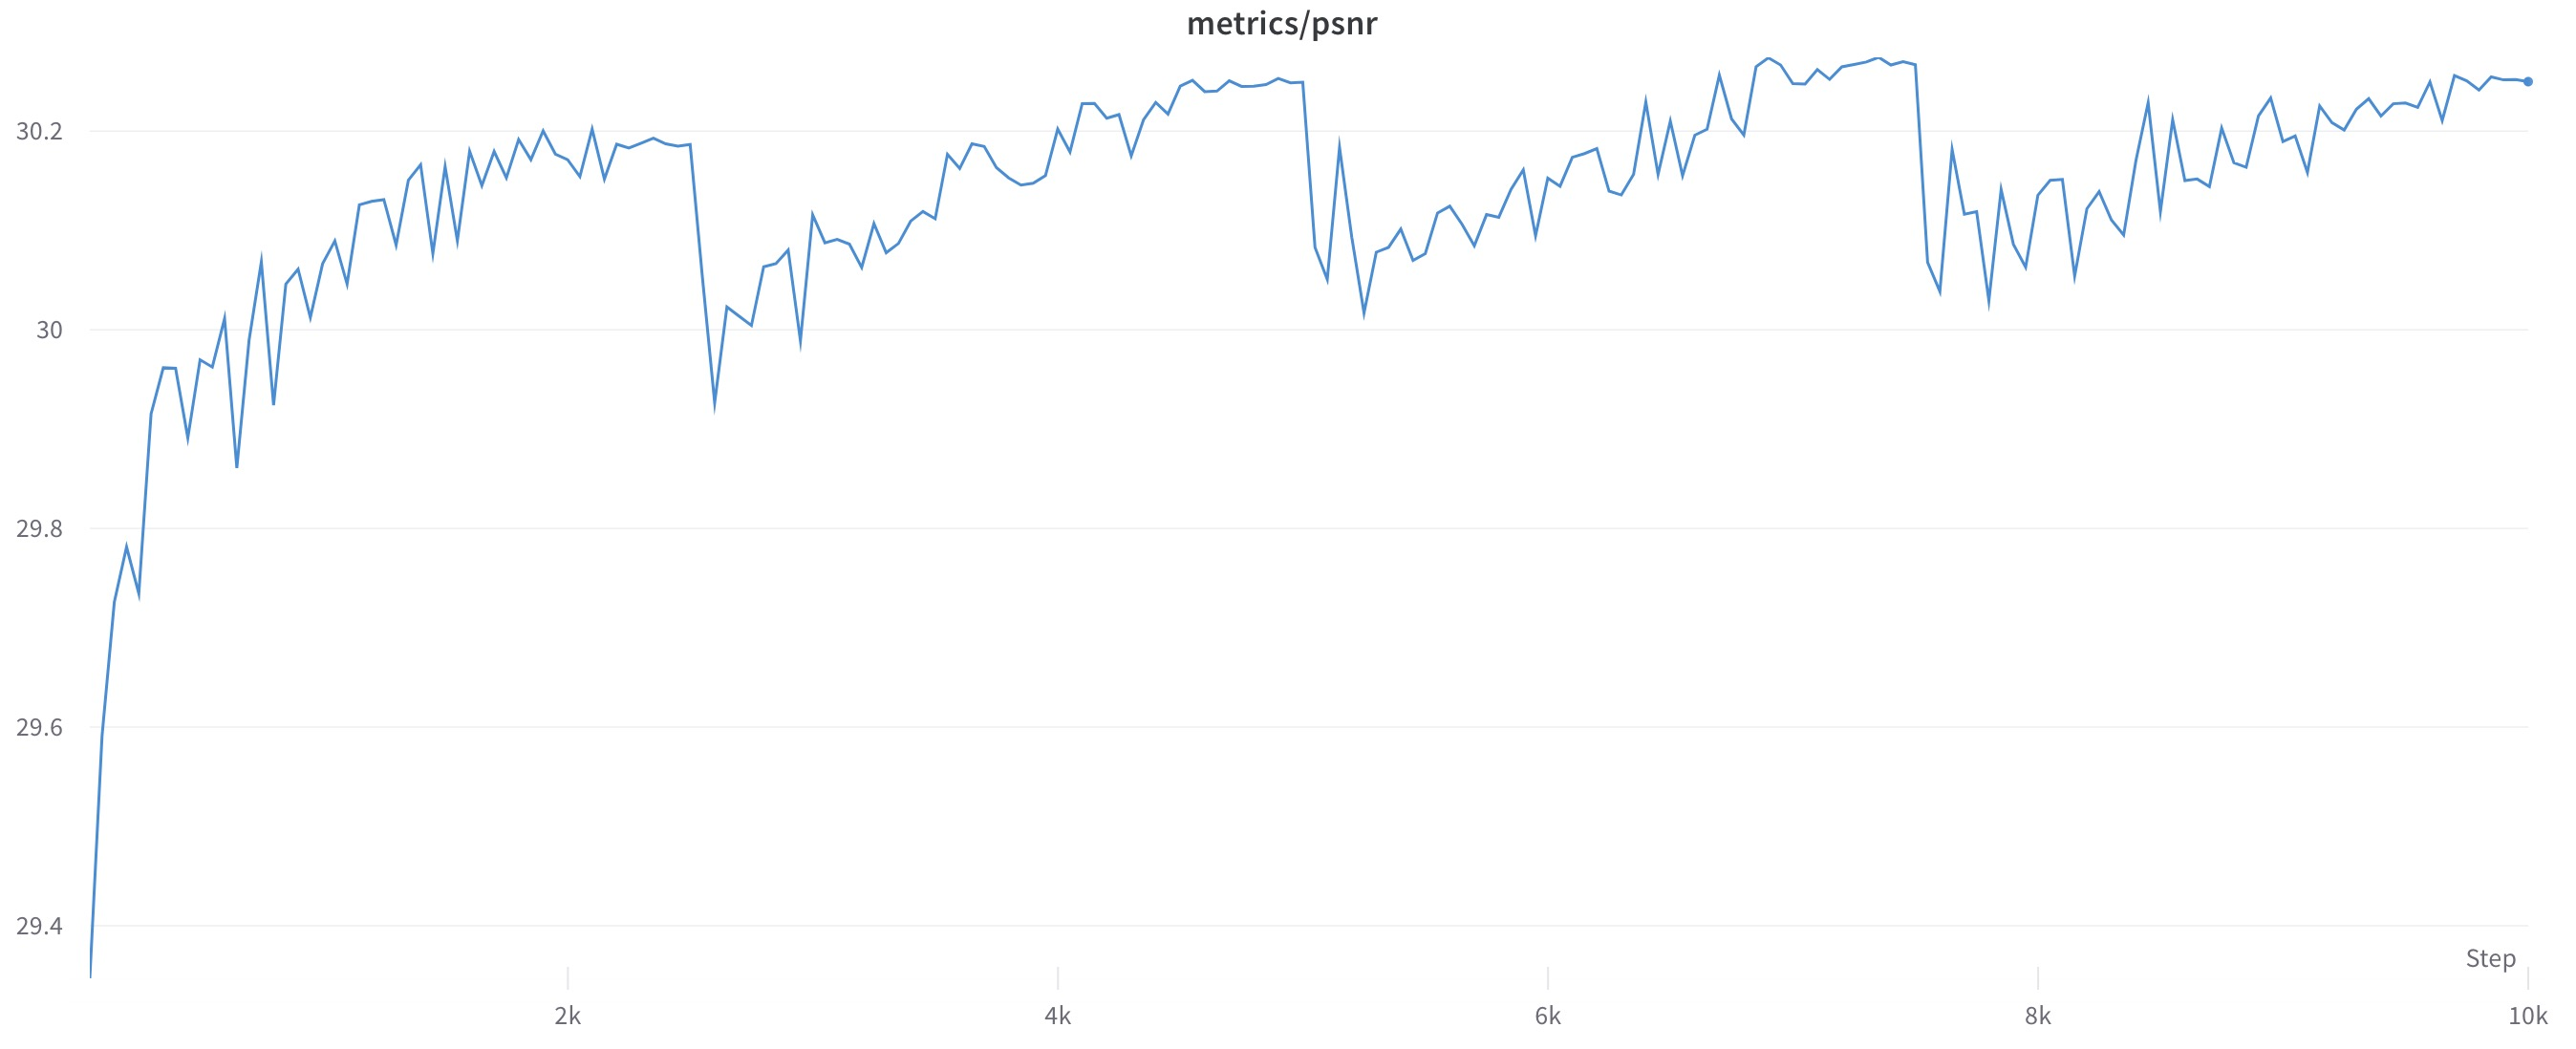
\includegraphics[width=\linewidth]{figures/SRResNet_psnr_curve.jpg}
          %         %\vspace{-1cm}
          %         \caption{SRResNet的PSNR训练曲线}
          %         %\label{fig:logo}
          %     \end{center}
          %     %\vspace{-0.7cm}
          % \end{figure}

          % 5. 测试过程,我们采用以下命令来对训练好的模型进行测试
          % \begin{minted}[xleftmargin=20pt,linenos,breaklines,bgcolor=bg]{python}
          % CUDA_VISIBLE_DEVICES=0 python basicsr/test.py -opt options/test/SRResNet_SRGAN/test_MSRResNet_x4.yml
          % \end{minted}

          % 其中,我们需要准备好待测数据集,比如test\_MSRResNet\_x4.yml配置文件中的DIV2K100测试集,需要我们按照第一步数据集准备的过程进行制作,然后设置对应路径

          % \begin{minted}[xleftmargin=20pt,linenos,breaklines,bgcolor=bg]{python}
          %   test_3:
          %     name: DIV2K100
          %     type: PairedImageDataset
          %     dataroot_gt: datasets/DIV2K/DIV2K_valid_HR
          %     dataroot_lq: datasets/DIV2K/DIV2K_valid_LR_bicubic/X4
          % \end{minted}

          % 此外,我们还需要对模型存放的路径进行设置
          % \begin{minted}[xleftmargin=20pt,linenos,breaklines,bgcolor=bg]{python}
          % path:
          %   pretrain_network_g: experiments/001_MSRResNet_x4_f64b16_DIV2K_1000k_B16G1_wandb/
          %   models/net_g_1000000.pth
          % \end{minted}

          % 设置完成后执行测试命令就可以在results文件夹下得到测试的结果图和PSNR等定量的指标结果。

\end{enumerate}

% ------------------------------------------------------------------------------

\section{测试流程}

测试阶段,我们需要在终端输入命令来开始训练。
\begin{minted}[xleftmargin=20pt,linenos,breaklines,bgcolor=bg]{python}
CUDA_VISIBLE_DEVICES=0 python basicsr/test.py -opt options/test/SRResNet_SRGAN/test_MSRResNet_x4.yml
\end{minted}

其中test\_MSRResNet\_x4为yml配置文件,主要设置实验相关的超参数和相关的一些配置参数。

\begin{hl} % ---------------- Highlight block ---------------- %

    \textbf{测试注意事项}

    如果需要额外添加测试集,需要使用test\_x格式,下划线之后是测试集的编号

    路径需要设置为待测模型所在的路径

    suffix配置为存储图片的名字后缀,一般设置为这个方法的名字便于对比

    metrics里面设置需要的评价指标,PSNR,SSIM和NIQE等

    分布式测试命令可参考:
    \href{https://github.com/XPixelGroup/BasicSR/blob/master/docs/TrainTest.md}{分布式训练和测试命令}

\end{hl}





\begin{minted}[xleftmargin=20pt,linenos,bgcolor=bg]{python}

def test_pipeline(root_path):
    # 加载配置参数
    opt, _ = parse_options(root_path, is_train=False)
    torch.backends.cudnn.benchmark = True

    # 新建loggers并初始化
    make_exp_dirs(opt)
    log_file = osp.join(opt['path']['log'],
    f"test_{opt['name']}_{get_time_str()}.log")
    logger = get_root_logger(logger_name='basicsr',
    log_level=logging.INFO, log_file=log_file)
    logger.info(get_env_info())
    logger.info(dict2str(opt))

    # 创建测试集和dataloader
    test_loaders = []
    for _, dataset_opt in sorted(opt['datasets'].items()):
        test_set = build_dataset(dataset_opt)
        test_loader = build_dataloader(
            test_set, dataset_opt, num_gpu=opt['num_gpu'],
            dist=opt['dist'], sampler=None, seed=opt['manual_seed'])
        logger.info(f"Number of test images in {dataset_opt['name']}:
        {len(test_set)}")
        test_loaders.append(test_loader)

    # 创建模型
    model = build_model(opt)
    # 测试多个测试集
    for test_loader in test_loaders:
        test_set_name = test_loader.dataset.opt['name']
        logger.info(f'Testing {test_set_name}...')
        model.validation(test_loader, current_iter=opt['name'],
        tb_logger=None, save_img=opt['val']['save_img'])


if __name__ == '__main__':
    root_path = osp.abspath(osp.join(__file__, osp.pardir, osp.pardir))
    test_pipeline(root_path)
\end{minted}

% ------------------------------------------------------------------------------

\section{推理流程}

快速推理阶段,我们需要在终端输入命令来进行快速推理:
\begin{minted}[xleftmargin=20pt,linenos,breaklines,bgcolor=bg]{python}
CUDA_VISIBLE_DEVICES=0 python basicsr/inference/inference_esrgan.py --input input_path --output out_path
\end{minted}

\begin{hl} % ---------------- Highlight block ---------------- %

    \textbf{推理注意事项}

    需要提前下载好预训练模型放在experiments/pretrained\_models/ 下面,在配置参数中可以详细的对比下载存放的路径和代码中设置的路径

    和测试不同,快速推理不涉及到定量评价指标的计算,比如PSNR,SSIM和NIQE等

    分布式测试命令可参考:
    \href{https://github.com/XPixelGroup/BasicSR/blob/master/docs/TrainTest.md}{分布式训练和测试命令}

\end{hl}



\begin{minted}[xleftmargin=20pt,linenos,breaklines,bgcolor=bg]{python}

#加载配置参数
parser = argparse.ArgumentParser()
parser.add_argument(
    '--model_path',
    type=str,
    default=  # noqa: E251
    'experiments/pretrained_models/ESRGAN/
    ESRGAN_SRx4_DF2KOST_official-ff704c30.pth'  # noqa: E501
)
parser.add_argument('--input', type=str,
default='datasets/Set14/LRbicx4', help='input test image folder')
parser.add_argument('--output', type=str, default='results/ESRGAN',
help='output folder')
args = parser.parse_args()

device = torch.device('cuda' if torch.cuda.is_available() else 'cpu')
# 设置快速推理所需要模型
model = RRDBNet(num_in_ch=3, num_out_ch=3, num_feat=64,
num_block=23, num_grow_ch=32)
model.load_state_dict(torch.load(args.model_path)['params'], strict=True)
model.eval()
model = model.to(device)

# 设置快速推理后输出的存放路径
os.makedirs(args.output, exist_ok=True)
for idx, path in enumerate(sorted(glob.glob(os.path.join(args.input, '*')))):
    imgname = os.path.splitext(os.path.basename(path))[0]
    print('Testing', idx, imgname)
    # 读取图片
    img = cv2.imread(path, cv2.IMREAD_COLOR).astype(np.float32) / 255.
    img = torch.from_numpy(np.transpose(img[:, :, [2, 1, 0]], (2, 0, 1))).float()
    img = img.unsqueeze(0).to(device)
    # 快速推理
    try:
        with torch.no_grad():
            output = model(img)
    except Exception as error:
        print('Error', error, imgname)
    else:
        # 保存图片
        output = output.data.squeeze().float().cpu().clamp_(0, 1).numpy()
        output = np.transpose(output[[2, 1, 0], :, :], (1, 2, 0))
        output = (output * 255.0).round().astype(np.uint8)
        cv2.imwrite(os.path.join(args.output, f'{imgname}_ESRGAN.png'), output)
\end{minted}

% ------------------------------------------------------------------------------

\section{入门样例}

这个部分我们以一个基础的超分模型SRResNet作为例子来展示BasicSR的入门使用。相关的文件目录如下所示:

\dirtree{%
    .1 \textcolor{black}{BasicSR}.
    .2 \textcolor{red}{basicsr}\DTcomment{BasicSR核心代码包}.
    .2 scripts\DTcomment{常用脚本}.
    .3 data\_preparation\DTcomment{数据准备脚本目录}.
    .4 extract\_subimages.py\DTcomment{生成子图脚本}.
    .2 datasets\DTcomment{数据集存放,推荐soft link}.
    .3 DIV2K\DTcomment{训练数据集}.
    .4 DIV2K\_train\_HR\_sub\DTcomment{训练数据集的GT子图}.
    .4 DIV2K\_train\_LR\_bicubic\_X4\_sub\DTcomment{训练数据集子图的下采样图}.
    .3 Set5\DTcomment{验证集}.
    .4 GTmod12\DTcomment{验证集的GT图}.
    .4 LRbicx4\DTcomment{验证集的下采样图}.
    .3 Set14\DTcomment{验证集}.
    .4 GTmod12\DTcomment{验证集的GT图}.
    .4 LRbicx4\DTcomment{验证集的下采样图}.
    .2 experiments\DTcomment{实验保存路径}.
    .3 pretrained\_models\DTcomment{预训练模型保存路径}.
    .3 001\_MSRResNet\_x4\_f64b16\_DIV2K\_1000k\_B16G1\_wandb\DTcomment{SRResNet实验存放路径}.
    .4 models\DTcomment{SRResNet训练模型存放位置}.
    .4 visualization\DTcomment{SRResNet实验验证图像}.
    .4 training\_states\DTcomment{SRResNet实验resume文件存放路径}.
    .4 001\_MSRResNet\_x4\_f64b16\_DIV2K\_1000k\_B16G1\_wandb\DTcomment{SRResNet实验配置文件}.
    .2 inference\DTcomment{快速推理获得结果}.
    .2 options\DTcomment{训练和测试配置文件}.
    .3 train\DTcomment{训练配置文件夹}.
    .4 SRResNet\_SRGAN\DTcomment{SRResNet训练配置文件夹}.
    .5 train\_MSRResNet\_x4.yml\DTcomment{SRResNet训练配置文件}.
    .3 test\DTcomment{测试配置文件夹}.
    .4 SRResNet\_SRGAN\DTcomment{SRResNet测试配置文件夹}.
    .5 test\_MSRResNet\_x4.yml\DTcomment{SRResNet测试配置文件}.
    % .4 train\_MSRResNet_x4.yml\DTcomment{SRResNet配置文件}.
    % .2 \textcolor{red}{scripts}\DTcomment{功能脚本,包含数据集制作,指标测试和数据集下载等}.
}

\begin{enumerate}

    \item 第一步是下载训练所用的数据集,常用的数据集链接可以参考:
          \href{https://github.com/XPixelGroup/BasicSR/blob/master/docs/DatasetPreparation.md#DIV2K}{https://github.com/XPixelGroup/BasicSR/blob/master/docs/DatasetPreparation.md\#DIV2K}

          在这里我们采用DIV2K 作为训练数据集,Set5作为验证集

          \begin{exampleBox}[]{数据集链接}

              DIV2K:
              \href{https://data.vision.ee.ethz.ch/cvl/DIV2K/}{https://data.vision.ee.ethz.ch/cvl/DIV2K/}

              Set5和Set14:
              \href{https://drive.google.com/drive/folders/1B3DJGQKB6eNdwuQIhdskA64qUuVKLZ9u}{https://drive.google.com/drive/folders/1B3DJGQKB6eNdwuQIhdskA64qUuVKLZ9u}

          \end{exampleBox}

          将下载好的训练集和验证集放在datasets目录下。(软链接是更好的方式,这里为了进行入门样例展示,采用了直接存放数据集的方式)

    \item 第二步是将下载好的DIV2K数据集切成子图的形式存放在DIV2K\_train\_HR\_sub目录下,由于2K图像的读取会占用大量的时间所以采用子图的形式进行读入

          \href{https://github.com/XPixelGroup/BasicSR/blob/master/scripts/data_preparation/extract_subimages.py}{https://github.com/XPixelGroup/BasicSR/blob/master/scripts/data\_preparation/extract\_subimages.py}

          \begin{minted}[xleftmargin=20pt,linenos,breaklines,bgcolor=bg]{python}

    # HR images 这个过程将2K的图像给切成480X480的子图
    # 原始2K图像路径
    opt['input_folder'] = 'datasets/DIV2K/DIV2K_train_HR'
    # 子图存放路径
    opt['save_folder'] = 'datasets/DIV2K/DIV2K_train_HR_sub'
    opt['crop_size'] = 480 # 子图的尺寸
    opt['step'] = 240 # 切图的步长
    opt['thresh_size'] = 0
    extract_subimages(opt)

    # LRx4 images
    opt['input_folder'] = 'datasets/DIV2K/DIV2K_train_LR_bicubic/X4'
    opt['save_folder'] = 'datasets/DIV2K/DIV2K_train_LR_bicubic/X4_sub'
    opt['crop_size'] = 120 # 子图的尺寸
    opt['step'] = 60 # 切图的步长

\end{minted}

    \item 制作好数据之后,修改yml配置文件中训练集和验证集的路径,就可以初步的把实验配置完成了

          % \begin{exampleBox}[]{配置文件修改}

          %     dataroot_gt: datasets/DF2K/DIV2K_train_HR_sub
          %     dataroot_lq: datasets/DF2K/DIV2K_train_LR_bicubic_X4_sub

          % \end{exampleBox}

          \begin{minted}[xleftmargin=20pt,linenos,breaklines,bgcolor=bg]{python}

# dataroot_gt: datasets/DF2K/DIV2K_train_HR_sub
# dataroot_lq: datasets/DF2K/DIV2K_train_LR_bicubic_X4_sub
# DF2K是DIV2K和Flickr2K数据集合并的数据集,这里我们先用DIV2K进行实验,可以根据需求调整自己的数据集
dataroot_gt: datasets/DIV2K/DIV2K_train_HR_sub
dataroot_lq: datasets/DIV2K/DIV2K_train_LR_bicubic_X4_sub

\end{minted}

    \item 训练命令和log显示

          \begin{minted}[xleftmargin=20pt,linenos,breaklines,bgcolor=bg]{python}
python basicsr/train.py -opt options/train/SRResNet_SRGAN/train_MSRResNet_x4.yml
\end{minted}

          执行训练命令之后,终端会打印出训练的相关信息和验证集上的PSNR的精度,如下所示:

          \begin{minted}[xleftmargin=20pt,linenos,breaklines,bgcolor=bg]{python}

2020-08-21 00:13:08,623 INFO: [001_M..][epoch:  4, iter:1,000,000, lr:(1.000e-07,)] [eta: 0:00:00, time (data): 0.041 (0.000)] l_pix: 2.1622e-02
2020-08-21 00:13:08,624 INFO: Saving models and training states.
... ...
Test head
[>>>>>>>>>>>>>>>>>>>>>>>>>>>>>>>>>>>>>>>>>>>>>>>>>>] 5/5, 21.3 task/s, elapsed: 0s, ETA:     0s
Test woman
2020-08-21 00:13:08,926 INFO: Validation Set5
 # psnr: 30.2497

\end{minted}

          同时,我们配置了wandb之后,可以在自己的wandb云端主页上看到训练曲线,wandb的配置见xx
          \begin{figure}[h]
              \vspace{1cm}
              \begin{center}
                  %\fbox{\rule{0pt}{2.5in} \rule{0.9\linewidth}{0pt}}
                  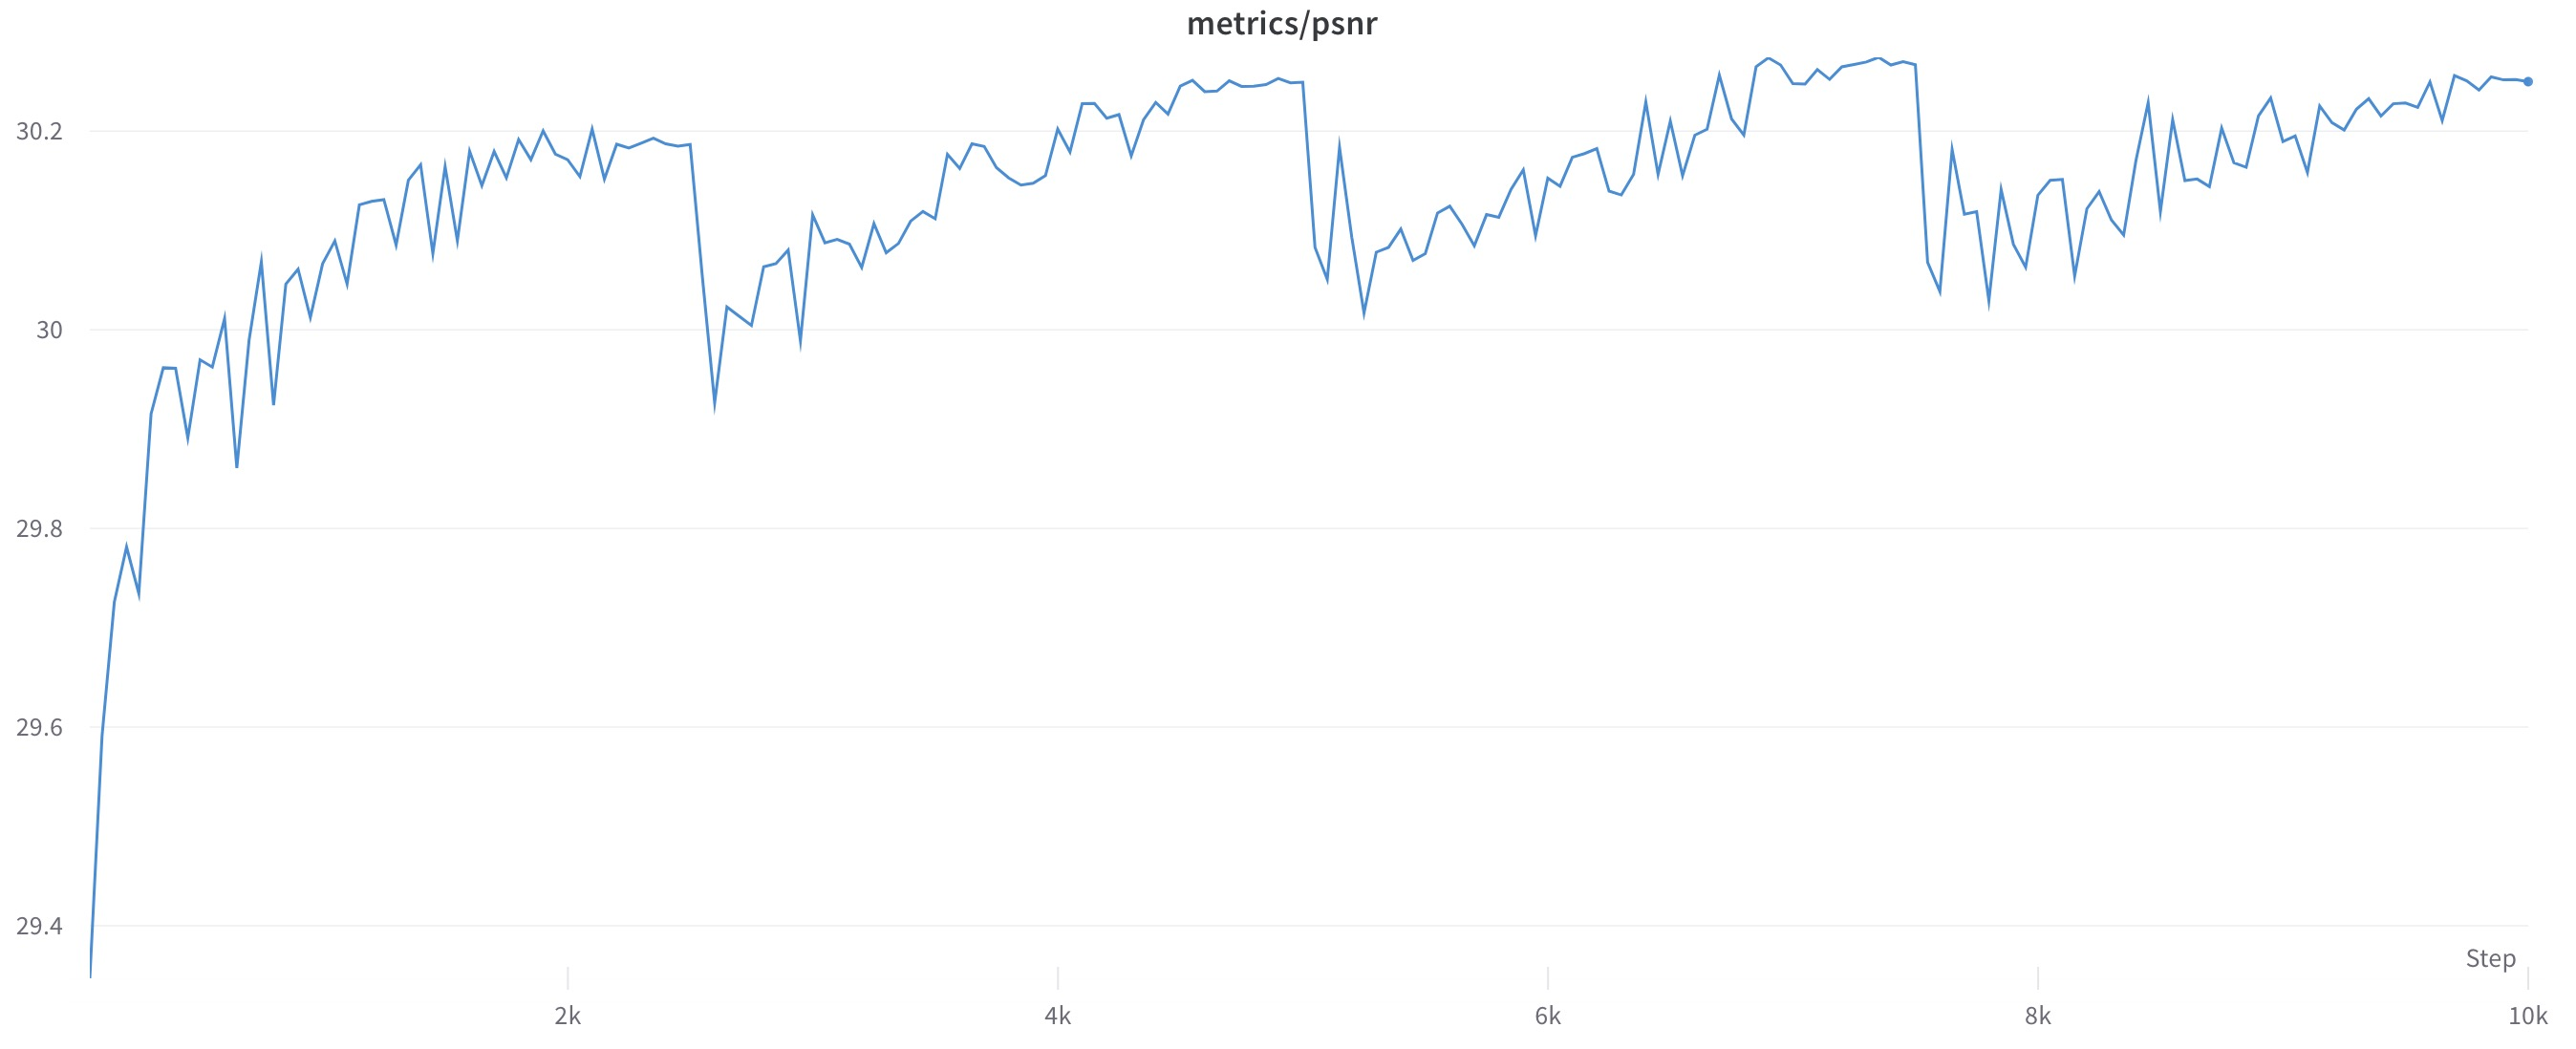
\includegraphics[width=\linewidth]{figures/SRResNet_psnr_curve.jpg}
                  %\vspace{-1cm}
                  \caption{SRResNet的PSNR训练曲线}
                  %\label{fig:logo}
              \end{center}
              %\vspace{-0.7cm}
          \end{figure}

          5. 测试过程,我们采用以下命令来对训练好的模型进行测试
          \begin{minted}[xleftmargin=20pt,linenos,breaklines,bgcolor=bg]{python}
CUDA_VISIBLE_DEVICES=0 python basicsr/test.py -opt options/test/SRResNet_SRGAN/test_MSRResNet_x4.yml
\end{minted}

          其中,我们需要准备好待测数据集,比如test\_MSRResNet\_x4.yml配置文件中的DIV2K100测试集,需要我们按照第一步数据集准备的过程进行制作,然后设置对应路径

          \begin{minted}[xleftmargin=20pt,linenos,breaklines,bgcolor=bg]{python}
  test_3:
    name: DIV2K100
    type: PairedImageDataset
    dataroot_gt: datasets/DIV2K/DIV2K_valid_HR
    dataroot_lq: datasets/DIV2K/DIV2K_valid_LR_bicubic/X4
\end{minted}

          此外,我们还需要对模型存放的路径进行设置
          \begin{minted}[xleftmargin=20pt,linenos,breaklines,bgcolor=bg]{python}
path:
  pretrain_network_g: experiments/001_MSRResNet_x4_f64b16_DIV2K_1000k_B16G1_wandb/
  models/net_g_1000000.pth
\end{minted}

          设置完成后执行测试命令就可以在results文件夹下得到测试的结果图和PSNR等定量的指标结果。

\end{enumerate}

\end{document}